%\documentclass[trans]{beamer}
\documentclass[9pt]{beamer}

% Try the class options [notes], [notes=only], [trans], [handout],
% [red], [compress], [draft], [class=article] and see what happens!

% Copyright 2003 by Till Tantau <tantau@users.sourceforge.net>.
%
% This program can be redistributed and/or modified under the terms
% of the LaTeX Project Public License Distributed from CTAN
% archives in directory macros/latex/base/lppl.txt.

% For a green structure color use:
%\colorlet{structure}{green!50!black}

%%%%%%%%%% User macros%%%%%%%%%%%
\newcommand{\mypurple}[1]{{\color[rgb]{0.7,0,0.8}#1}}
\newcommand{\myred}  [1] {{\color{red}#1}}
\newcommand{\myblue} [1] {{\color{blue}#1}}
\newcommand{\mygreen}[1] {{\color[rgb]{0,0.5,0}#1}}
\newcommand{\Nat}{\mathbb{N}}
\def\sla  {\!\!\!\slash}
%%%%%%%%%%%%%%%%%%%%%%%%%%%%%%%%%
\mode<article> % only for the article version
{
  \usepackage{beamerbasearticle}
  \usepackage{fullpage}
  \usepackage{hyperref}
}

%\beamertemplateshadingbackground{red!10}{blue!10}
%\beamertemplateshadingbackground{blue!10}{blue!10}

%\usepackage{beamerthemeshadow}

\usepackage{pgf,pgfarrows,pgfnodes,pgfautomata,pgfheaps,pgfshade}
\usepackage{amsmath,amssymb}
\usepackage[latin1]{inputenc}
\usepackage{colortbl}
\usepackage[english]{babel}
%\usepackage{verbatim}
%\usepackage{listings}
\usepackage[procnames]{listings}

%\usepackage{lmodern}
\usepackage[T1]{fontenc} 

\usepackage{times}

% for code colouring
\include{pythonlisting}
\include{cpplisting}
%\usepackage{minted}

% Use some nice templates
\beamertemplatetransparentcovereddynamic
\usetheme{Binet}
%\usetheme{Madrid}
%\usetheme{Boadilla}
%\usetheme{Berkeley}
%\usetheme{Rochester}

%\def\command#1{\list{}{\leftmargin=2em\itemindent-\leftmargin\def\makelabel##1{\hss##1}}%
%\item\extractcommand#1@\par\topsep=0pt}
%\def\endcommand{\endlist}
%\def\extractcommand#1#2@{\strut\declare{\texttt{\string#1}}#2}

%
% The following info should normally be given in you main file:
%

\hypersetup{%
  pdftitle={Software in HEP:\\Parallelism strikes back},%
  pdfauthor={Sebastien Binet}
  %pdfsubject={AthenaMP},
  %pdfkeywords={ATLAS,Athena,python,COW,parallelization},
%  pdfpagemode=FullScreen%
}

\title[HEP sw]{Software in HEP:\\Parallelism strikes back}
\author[S. Binet]{S\'ebastien~Binet}%\inst{1}
\institute[LAL]{
%  \inst{1}%
  LAL/IN2P3}
\date{2014-11-20}

% \begin{center}
% On behalf of Core people
% \end{center}

\pgfdeclaremask{lal}{lal}
\pgfdeclareimage[mask=lal,width=2cm]{lal-logo}{lal}

\logo{%
  \vbox{%
    \hbox{\pgfuseimage{lal-logo}}%
  }%
}


\begin{document}
\lstset{language=C++}

\frame{\titlepage
%  \hskip0.44\paperwidth
%  \insertlogo

    \begin{beamercolorbox}[sep=8pt,center]{mylogo}
      \usebeamercolor[fg]{mylogo}\insertlogo
    \end{beamercolorbox}

}

%\section*{Outline}
%\frame{\tableofcontents[part=1]}%,pausesections]}

%\AtBeginSubsection[]
%{
%  \frame<handout:0>
%  {
%    \frametitle{Outline}
%    \tableofcontents[current,currentsubsection]
%  }
%}

\part<presentation>{Main Talk}

%%%%%%%%%%%%%%%%%%%%%%%%%%%%%%%%%%%%%%%%%%%%%%%%%%%%%%%%%%%%%%%%%%%%%%%%%%%%%%%
%%%%%%%%%%%%%%%%%%%%%%%%%%%%%%%%%%%%%%%%%%%%%%%%%%%%%%%%%%%%%%%%%%%%%%%%%%%%%%%
%\section[Outline]{Outline}

% \frame<beamer>{
%   \frametitle{Outline}
%   \begin{columns}
% \begin{column}{0.49\textwidth}
%   \begin{block}{}
%   \tableofcontents
%   \end{block}
% \end{column}
% \end{columns}

% }
%\frame{\partpage}

%%%%%%%%%%%%%%%%%%%%%%%%%%%%%%%%%%%%%%%%%%%%%%%%%%%%%%%%%%%%%%%%%%%%%%%%%%%%%%%
%%%%%%%%%%%%%%%%%%%%%%%%%%%%%%%%%%%%%%%%%%%%%%%%%%%%%%%%%%%%%%%%%%%%%%%%%%%%%%%
\section[mysection]{mysection}

\frame{
  \frametitle{Parallelism: why?}

  \begin{center}
    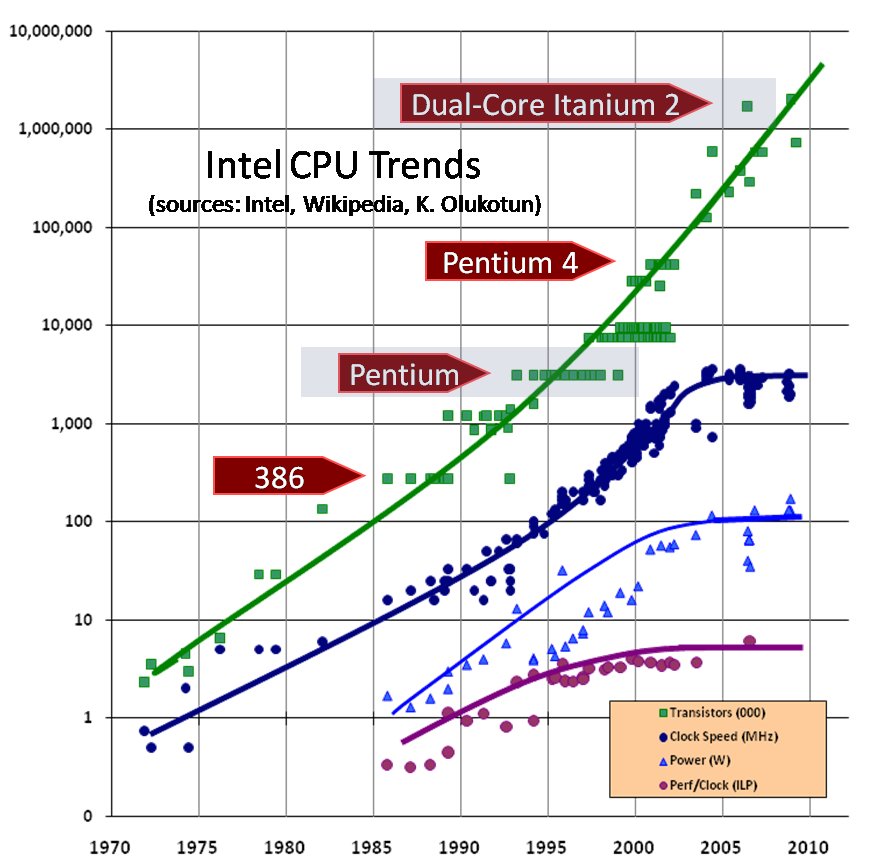
\includegraphics[width=0.65\textwidth]{figs/cpu-free-lunch.png}
  \end{center}
  
}

\frame{\frametitle{A bit of history: 1950-2000}
  \begin{itemize}
  \item \myred{1954:} computers were valve-based
  \item \myred{1956:} first magnetic disk system sold (IBM RAMAC)
  \item \myred{$\sim$ 1956:} \texttt{FORTRAN} under development
  \item \myred{1959:} IBM-1401 shipped. Transistorised. Punched card input.
  \item \myred{1960:} PDP-1 launched (18-bit words)
  \item \myred{1964:} PDP-8 launched (12-bit words)
  \item \myred{1964:} System/360 launched (4*8-bit byte words, 8-64-256 $kB$ of RAM)
    
  \end{itemize}

  \begin{center}
    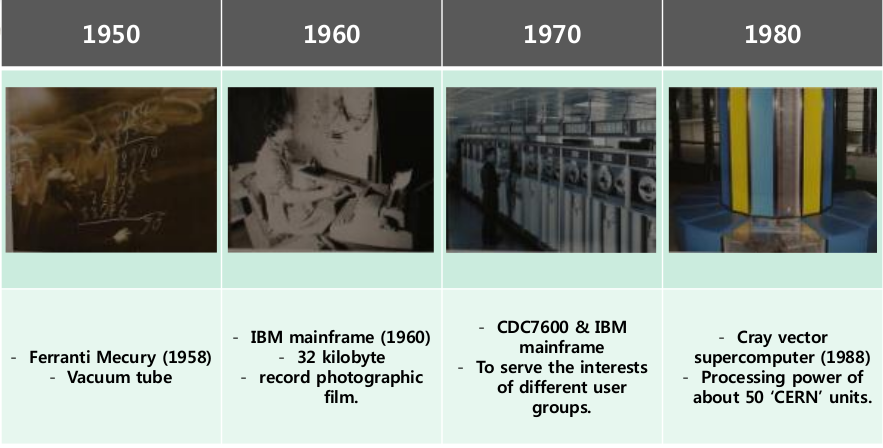
\includegraphics[width=0.68\textwidth]{figs/cern-computers.png}
    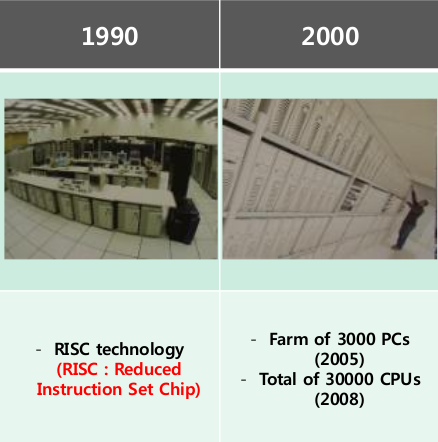
\includegraphics[width=0.34\textwidth]{figs/cern-computers-2000.png}
  \end{center}
}


\frame{\frametitle{A bit of history: 1950-2000 (at \texttt{CERN})}
  \begin{itemize}
  \item \myred{1963:} IBM-7090 ($\times 4$ \texttt{CERN} total computing capacity at the time)
  \item \myred{1965:} CDC-6600 ($1 MFLOPs$, $\times 15$ \texttt{CERN}'s capacity)
  \item \myred{1972-1984:} CDC-7600, IBM-370/168
  \item \myred{1982:} VAX 750s,780s,8600s
  \item \myred{1988-1993:} Cray
  \item \myred{1996:} \emph{mainframe rundown} completed. (mainframes
      replaced by \texttt{UNIX} and PC servers.)
  \end{itemize}

  \begin{center}
    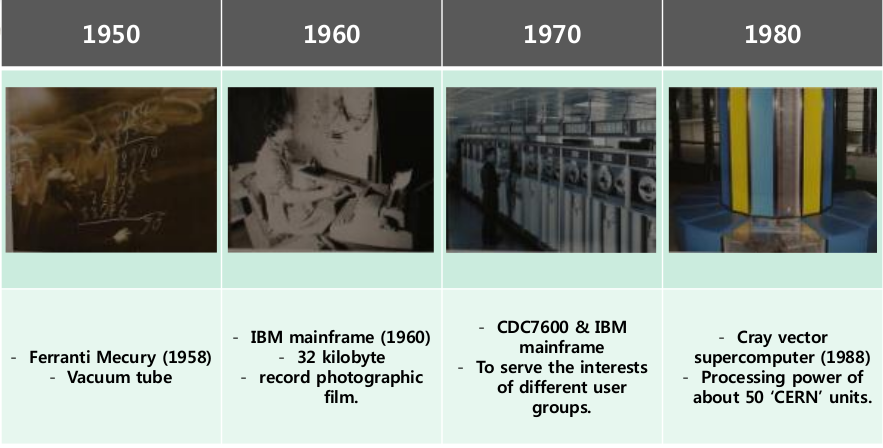
\includegraphics[width=0.68\textwidth]{figs/cern-computers.png}
    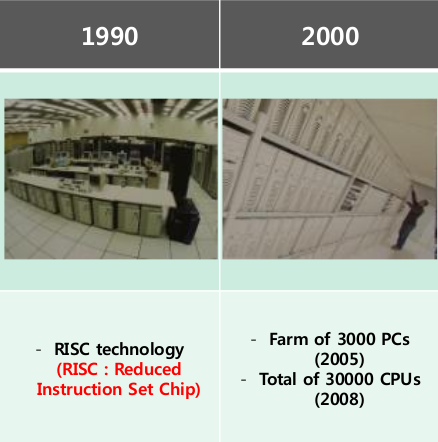
\includegraphics[width=0.34\textwidth]{figs/cern-computers-2000.png}
  \end{center}
}

\frame{
  \begin{center}
    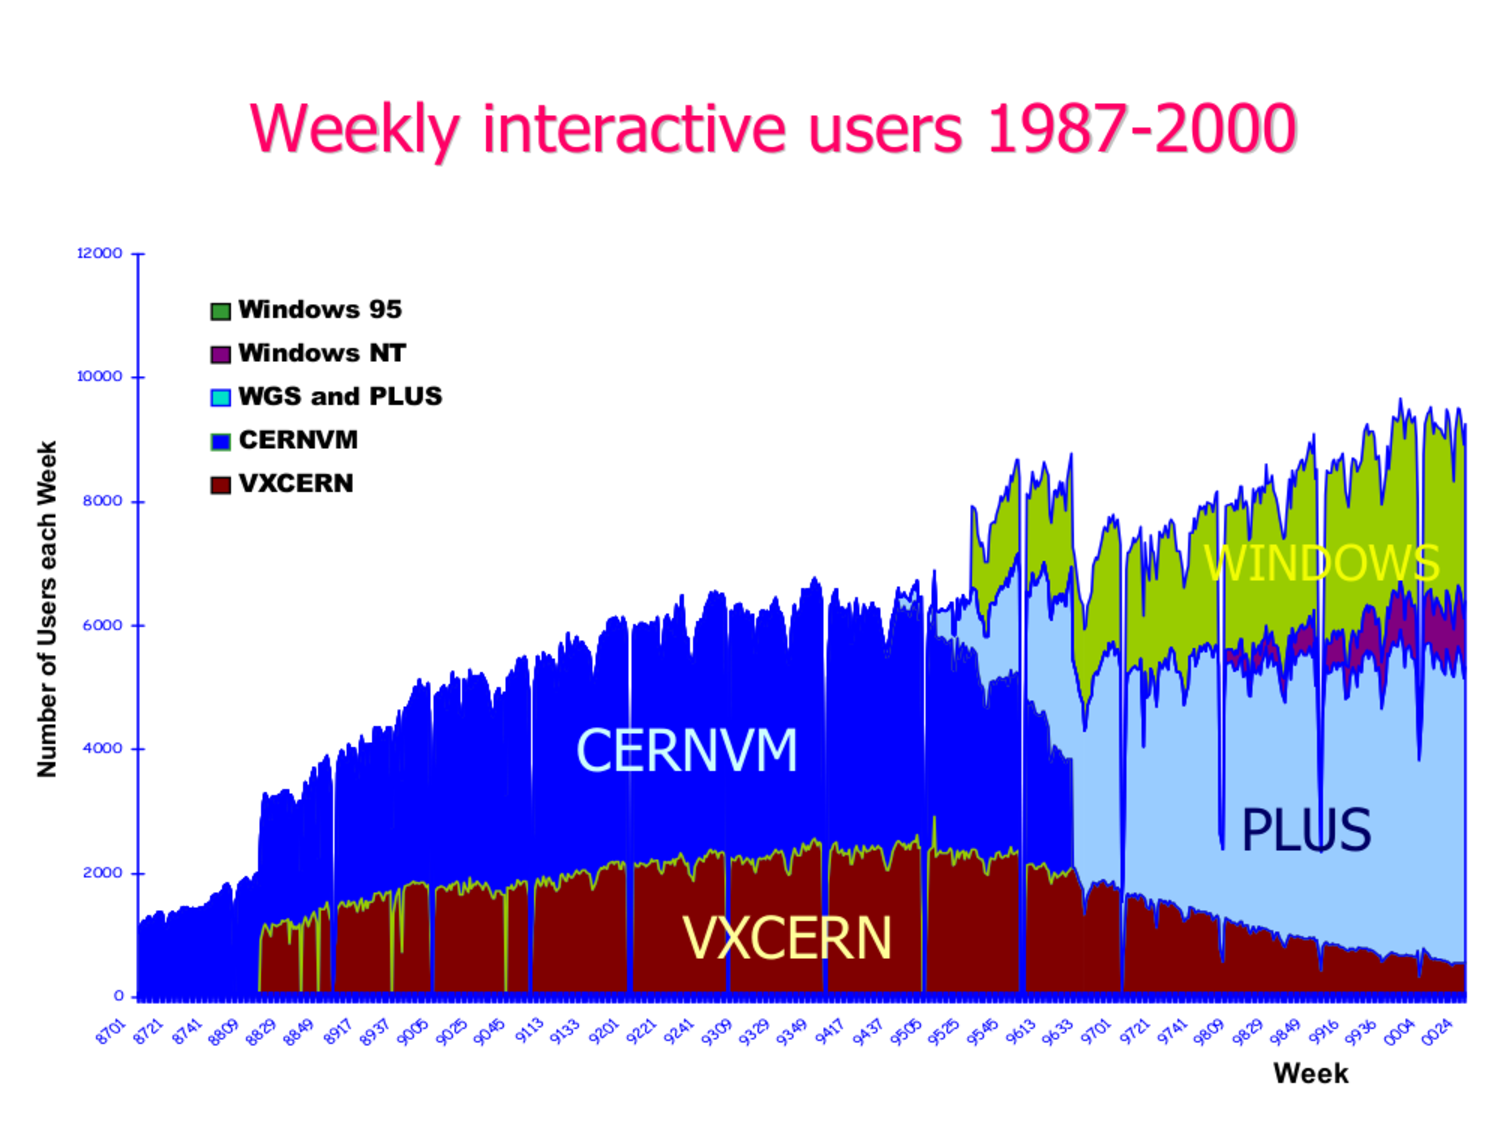
\includegraphics[width=0.95\textwidth]{figs/weekly-interactive-users.pdf}
  \end{center}
}

\frame{\frametitle{A bit of history: 1950-2000 in (offline) software}
  \begin{block}{}
  \begin{itemize}
  \item \myred{60's-00's:} \texttt{FORTRAN} is king
  \item \myred{1964:} \texttt{CERN} Programme Library
  \item \texttt{REAP} (paper tape measurements), \texttt{THRESH}
    (geometry reconstruction), \texttt{GRIND} (kinematic analysis), \texttt{SUMX}, \texttt{HBOOK} (statistical analysis chain),
  \item \texttt{PATCHY} (source code management),
  \item \texttt{ZEBRA} (memory management, I/O, \ldots),
  \item \texttt{GEANT3}, \texttt{PAW}
  \end{itemize}
  \end{block}

  \begin{exampleblock}{}
    \begin{itemize}
    \item \myred{mid-90's-\ldots:} \texttt{C++} takes roots in HEP
      \item Object Oriented programming is the cool kid on the block
      \item \texttt{Geant4}, \texttt{ROOT}, \texttt{POOL},
        \texttt{LHC++}, \texttt{AIDA}
    \end{itemize}
  \end{exampleblock}

  \begin{block}{}
  \begin{itemize}
    \item \myred{00's-\ldots:} \texttt{Python} becomes the
      \emph{de facto} scripting language in HEP
    \item framework data cards
    \item analysis glue, analyses in \texttt{python}
      \begin{itemize}
      \item \texttt{PyROOT}, \texttt{rootpy},
      \item \texttt{numpy}, \texttt{scipy}, \texttt{IPython}, \texttt{matplotlib}
      \end{itemize}      
  \end{itemize}
  \end{block}
}

\frame{\frametitle{Current software in a nutshell (\emph{e.g.:} \textsc{Atlas})}
  \begin{block}{}
  \begin{itemize}
    \item \mypurple{Generators:} generation of true particles from
      fondamental physics first principles,
      \begin{itemize}
        \item not easy, but no software challenge either
      \end{itemize}
    \item \mypurple{Full Simulation:} tracking of all stable
      particles in magnetic field through the detector simulating
      interaction, recording energy deposition (\myred{\texttt{CPU}
        intensive}),
    \item \mypurple{Reconstruction:} from real data as it comes
      out of the detector, or from \emph{Monte-Carlo} simulation
      data as above,
    \item \mypurple{Fast Simulation:} parametric simulation,
      faster, coarser,
    \item \mypurple{Analysis:} Daily work of physicists, running
      on output of reconstruction to derive analysis specific
      information (\myred{\texttt{I/O} intensive})
      \item everything in the same (\texttt{C++}) offline control framework (except analysis)
  \end{itemize}
  \end{block}

  \begin{center}
    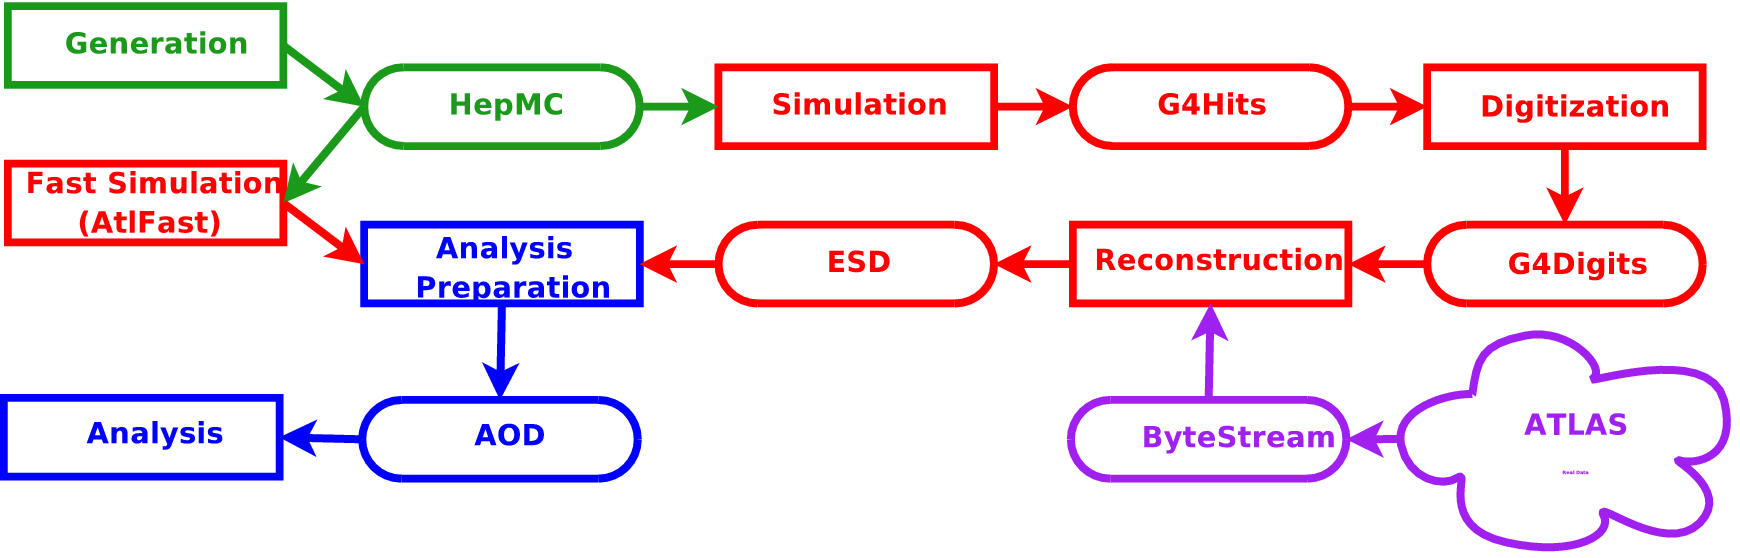
\includegraphics[width=0.95\textwidth]{figs/data-flux-summary-all.png}
  \end{center}
  %% \begin{block}{}
  %%   Everything in the same (offline control) framework, except for the
  %%   last analysis step (in \texttt{ROOT}).
  %% \end{block}
}

\frame{\frametitle{Offline frameworks (\textsc{Atlas, LHCb})}

  \begin{block}{}
    \texttt{Gaudi} is:
    \begin{itemize}
      \item a component object model (\texttt{COM}) based framework
      \item mainly written in \texttt{C++}
      \item with bits and pieces written in \texttt{python} for
        steering
      \item (although more and more pieces in \texttt{python} for
        analysis)
      \item most of the code written under a \emph{single thread}
        assumption
        \begin{itemize}
          \item most of the code is \mypurple{not thread safe}
        \end{itemize}
    \end{itemize}
  \end{block}

  \begin{center}
    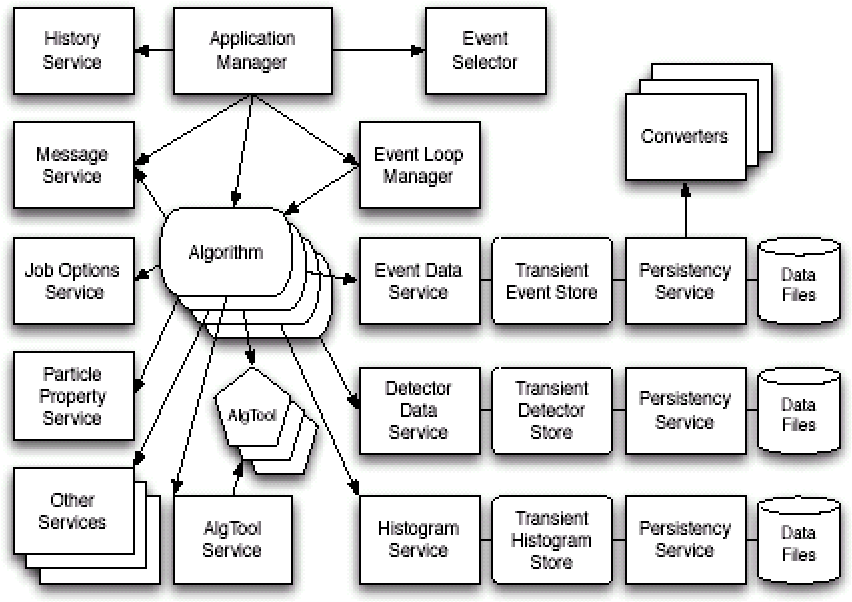
\includegraphics[width=0.5\linewidth]{figs/athena-component-model.pdf}
  \end{center}
}


\frame{\frametitle{Offline framework architecture: components \& black-board}
  \begin{center}
    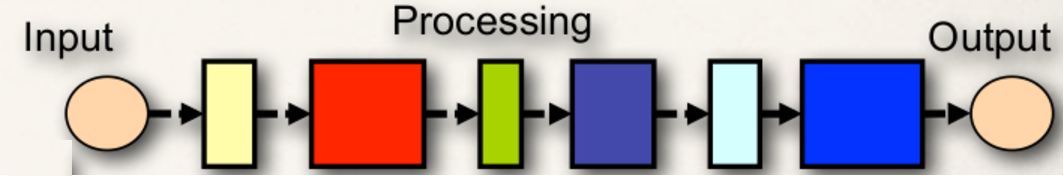
\includegraphics[width=0.85\textwidth]{figs/serial-processing.pdf}
  \end{center}
  \begin{center}
    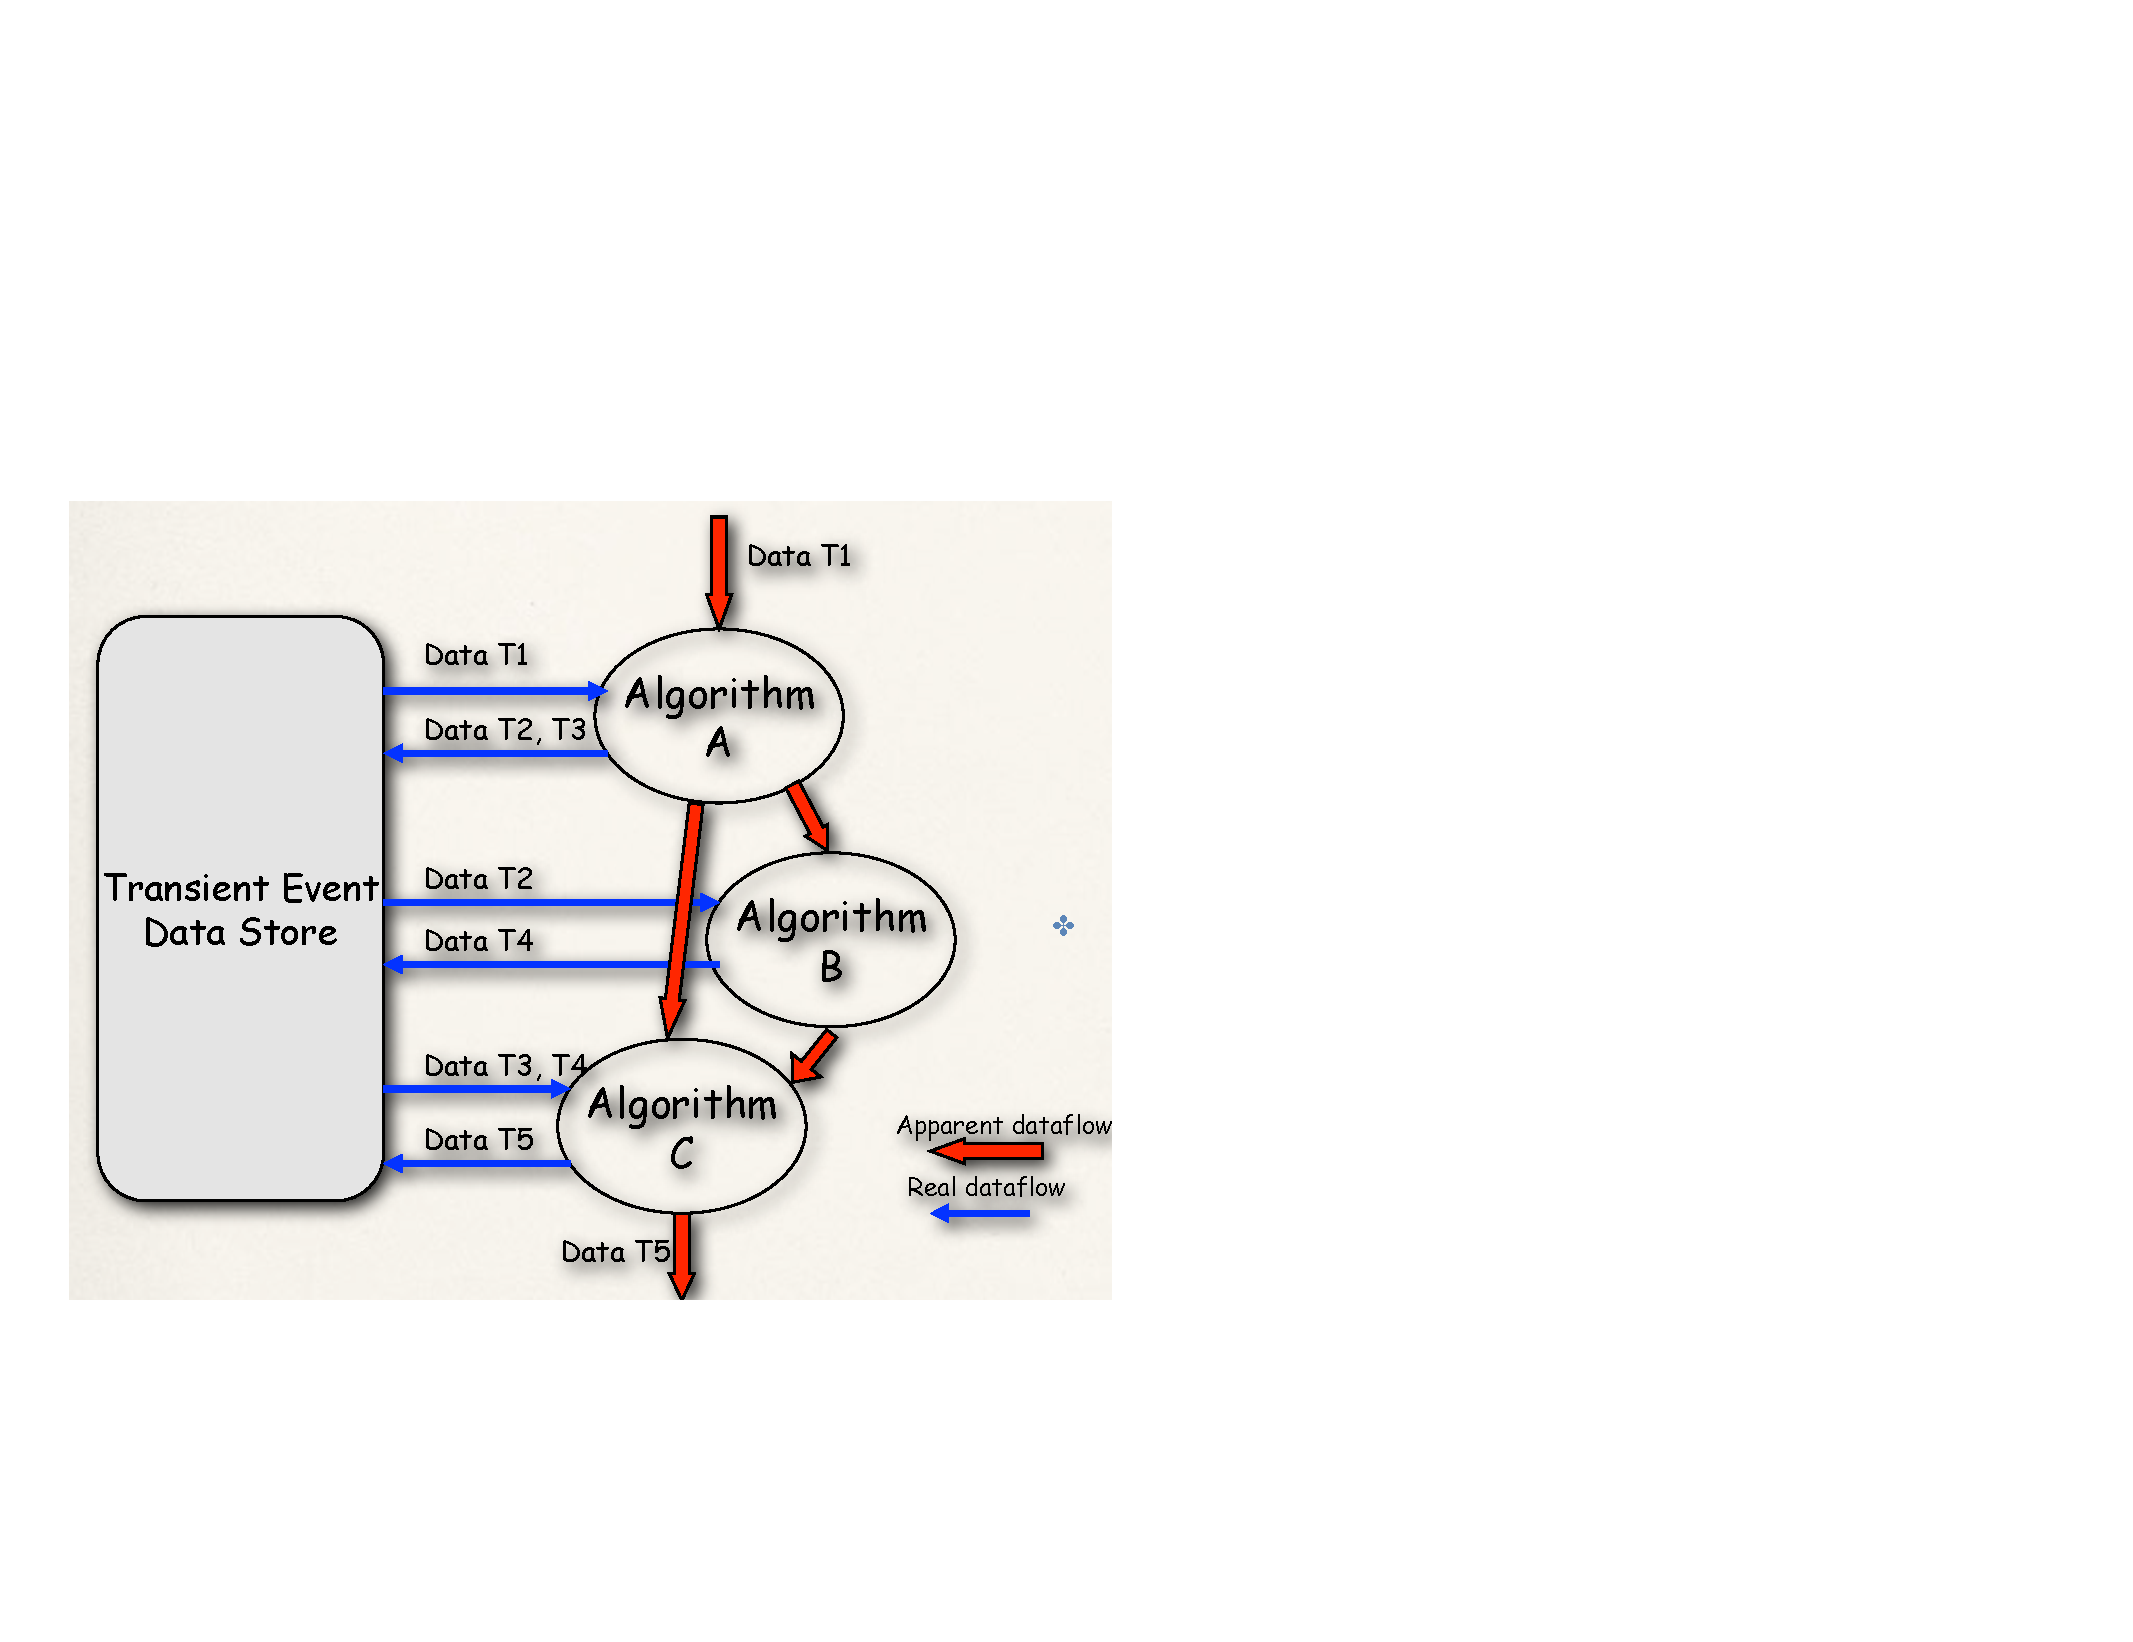
\includegraphics[width=0.65\textwidth]{figs/data-flow.pdf}
  \end{center}
}

\frame{\frametitle{Offline framework architecture: components \& black-board}
  \begin{center}
    \begin{figure}
    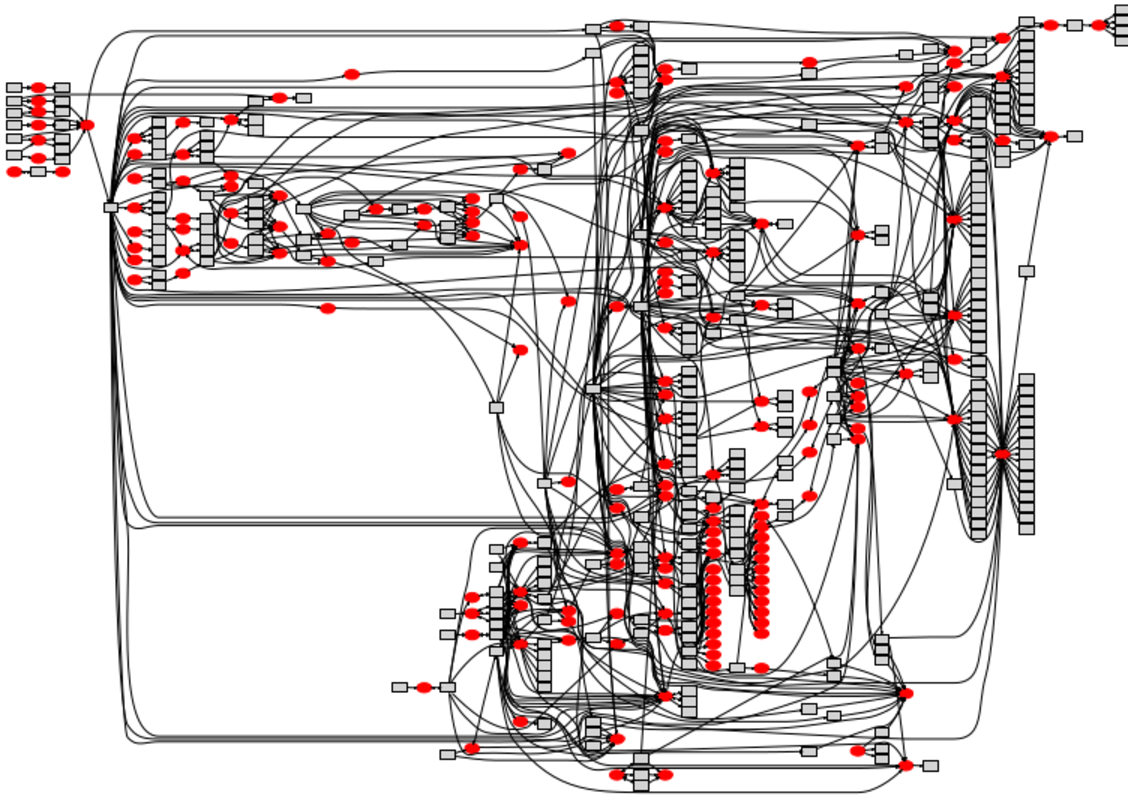
\includegraphics[width=0.85\textwidth]{figs/dag-comps-atlas.pdf}
    \caption{Directed acyclic graph of algorithms from a
      reconstruction job}
    \end{figure}
  \end{center}
}

\frame{\frametitle{Software in HEP: some numbers}

  \begin{block}{}
    \begin{itemize}
    \item Reconstruction frameworks grew from $\sim$3M \texttt{SLOC} to $\sim$ 5M
    \item Summing over all HEP software stack for e.g. \textsc{Atlas}:

      \begin{itemize}
      \item event generators: $\sim 1.4M$ \texttt{SLOC} (\texttt{C++}, \texttt{FORTRAN-77})
      \item  \texttt{I/O} libraries $\sim 1.7M$ \texttt{SLOC} (\texttt{C++})
      \item simulation libraries $\sim 1.2M$ \texttt{SLOC} (\texttt{C++})
      \item  reconstruction framework $\sim 5M$ \texttt{SLOC}
      \item  reconstruction steering/configuration ($\sim 1M$ \texttt{SLOC} \texttt{python})

      \end{itemize}

    \item \texttt{GCC}: $7M$ \texttt{SLOC}

    \item \texttt{Linux} kernel 3.6: $15.9M$ \texttt{SLOC}
    \end{itemize}
  \end{block}

}

\frame{\frametitle{Software development cycle}

  \begin{block}{}
    \begin{itemize}
    \item VCS (CVS, then SVN. GIT: not yet, at least not for \texttt{LHC} experiments)


    \item Nightlies (Jenkins or homegrown solution)
      \begin{itemize}
        \item need a sizeable cluster of build machines (\texttt{distcc}, \texttt{ccache}, ...)
        \item builds the framework stack in $\sim$8h
        \item produces $\sim$ 2000 shared libraries
        \item installs them on \texttt{AFS} (also creates \texttt{RPM}s and tarballs)
      \end{itemize}

    \item Devs can then test and develop off the nightly \emph{via} \texttt{AFS}
    \end{itemize}
  \end{block}

  \begin{exampleblock}{}
Every 6 months or so a new production release is cut, validated (then patched) and deployed on the World Wide LHC Computing Grid (\texttt{WLCG}).

\begin{itemize}
  \item Release size: \myred{$\sim$ 5Gb}
  \item binaries, libraries (externals+framework stack)
  \item  extra data (\texttt{SQLite} files, physics processes' modelisation data, \ldots)
\end{itemize}
  \end{exampleblock}

}

\frame{\frametitle{Software runtime ?}

  \begin{block}{}
    Big science, big data, big software, big numbers
    \begin{itemize}
    \item $\sim$ 1min to initialize the application
    \item loading >500 shared libraries
    \item connecting to databases (detector description, geometry, ...)
    \item instantiating $\sim$2000 \texttt{C++} components
    \item $2Gb/4Gb$ memory footprint per process
    \end{itemize}
  \end{block}

  \begin{center}

    \begin{figure}
      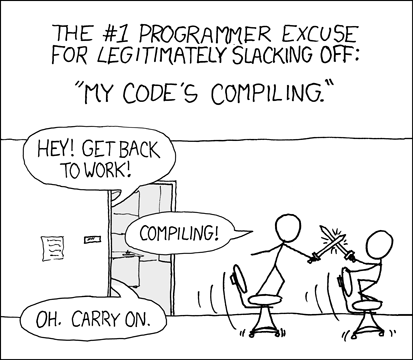
\includegraphics[width=0.4\textwidth]{figs/xkcd-compiling.png}
    \end{figure}
    (obligatory \texttt{xkcd} reference)
  \end{center}
  
}

\frame{\frametitle{Software in HEP: sustainable development ?}
  \begin{block}{}
    \begin{itemize}
    \item People committing code to VCS per month
      \begin{itemize}
      \item Wide variety of skill level
      \item Large amount of churn
      \item Once the physics data is pouring, people go and do physics instead of software
      \end{itemize}
    \end{itemize}
  \end{block}

  \begin{columns}
    \begin{column}{0.5\textwidth}

      \begin{center}
        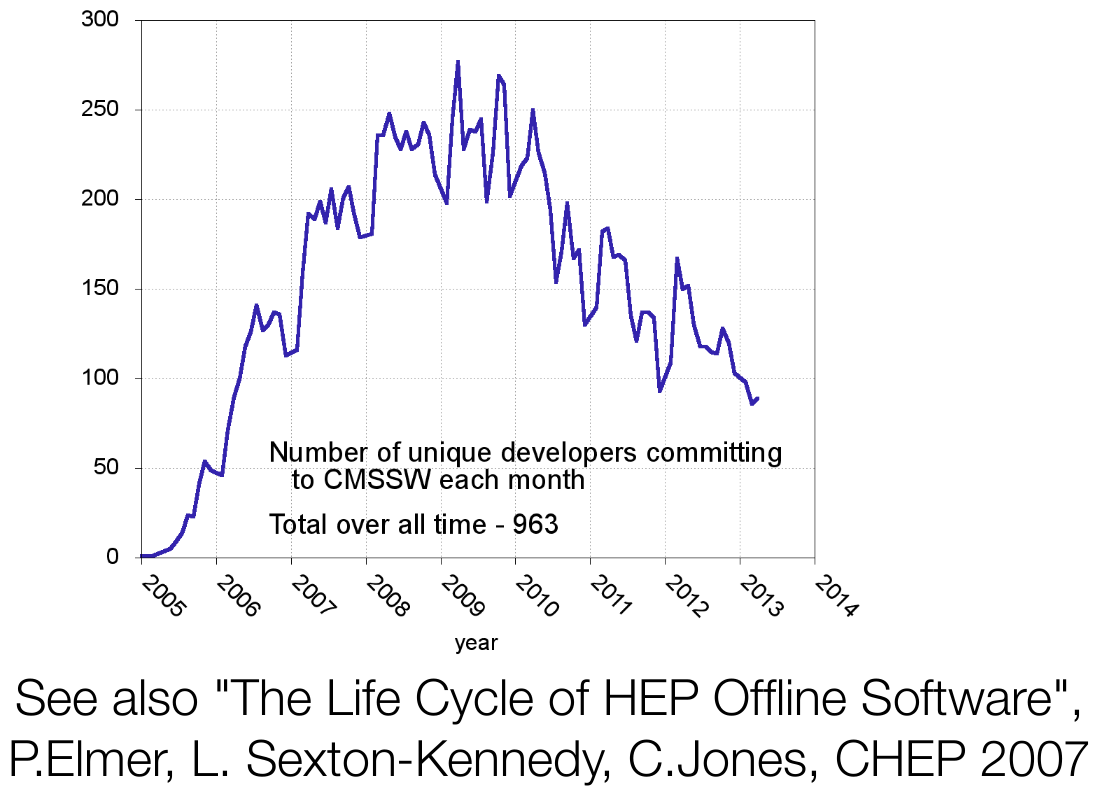
\includegraphics[width=0.99\textwidth]{figs/cmssw-commits.png}
      \end{center}
    \end{column}
    \begin{column}{0.5\textwidth}

      \begin{center}
        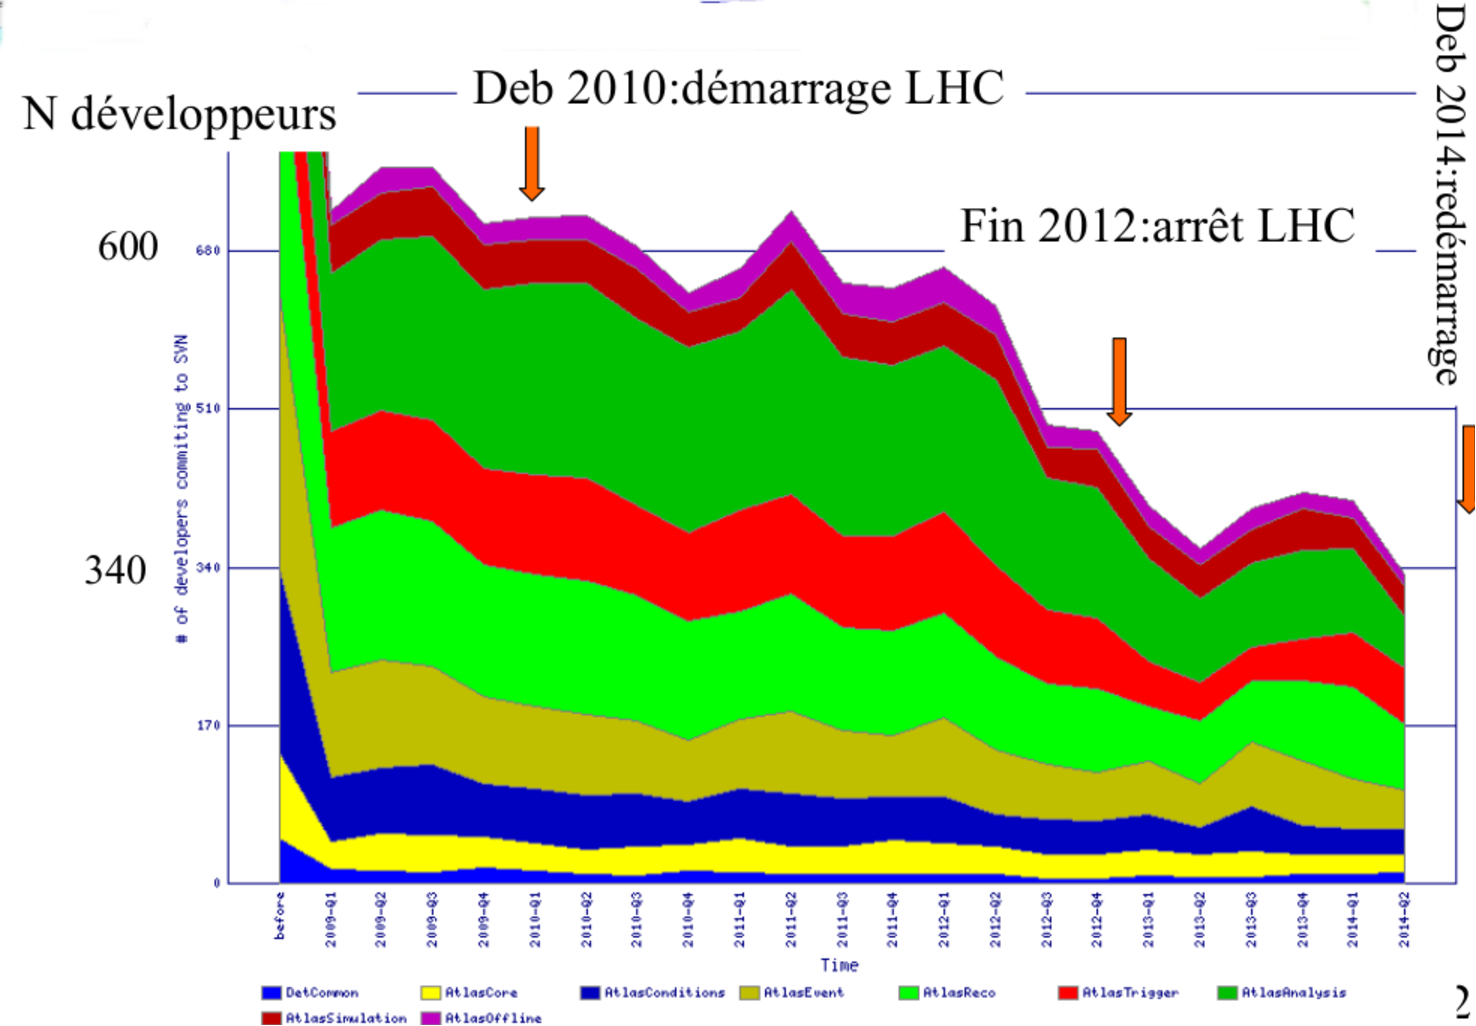
\includegraphics[width=0.99\textwidth]{figs/atlassw-commits.pdf}
      \end{center}
    \end{column}
  \end{columns}
  
}

\frame{\frametitle{Moore's law}
  \begin{center}
    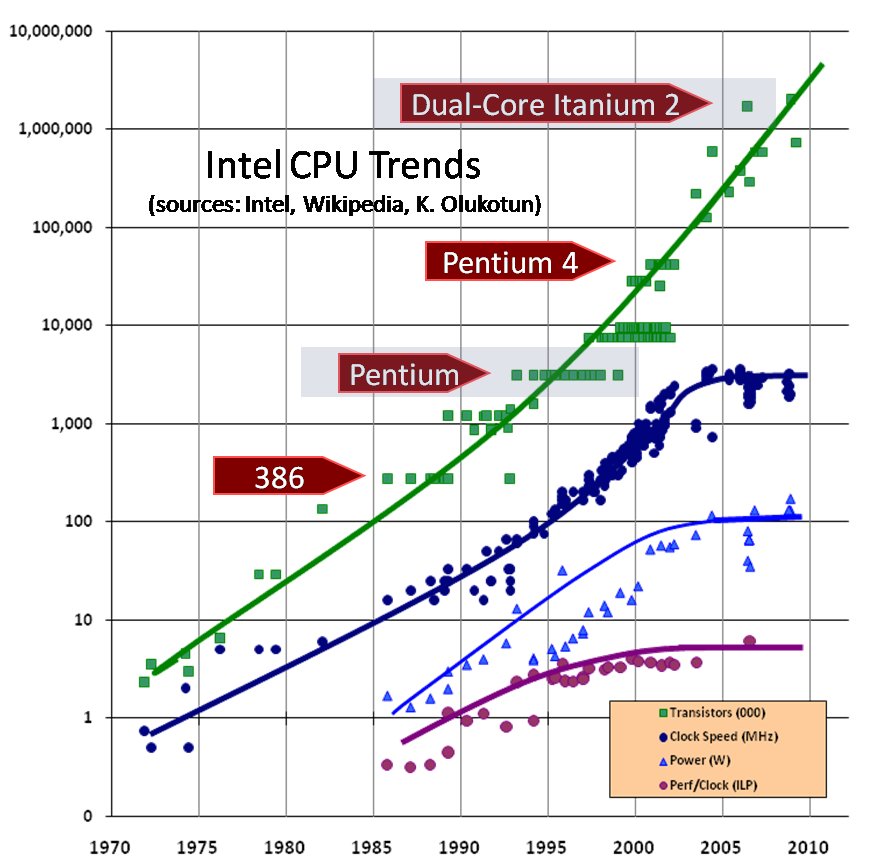
\includegraphics[width=0.65\textwidth]{figs/cpu-free-lunch.png}
  \end{center}
}

\frame{\frametitle{Moore's law}
  \begin{center}
    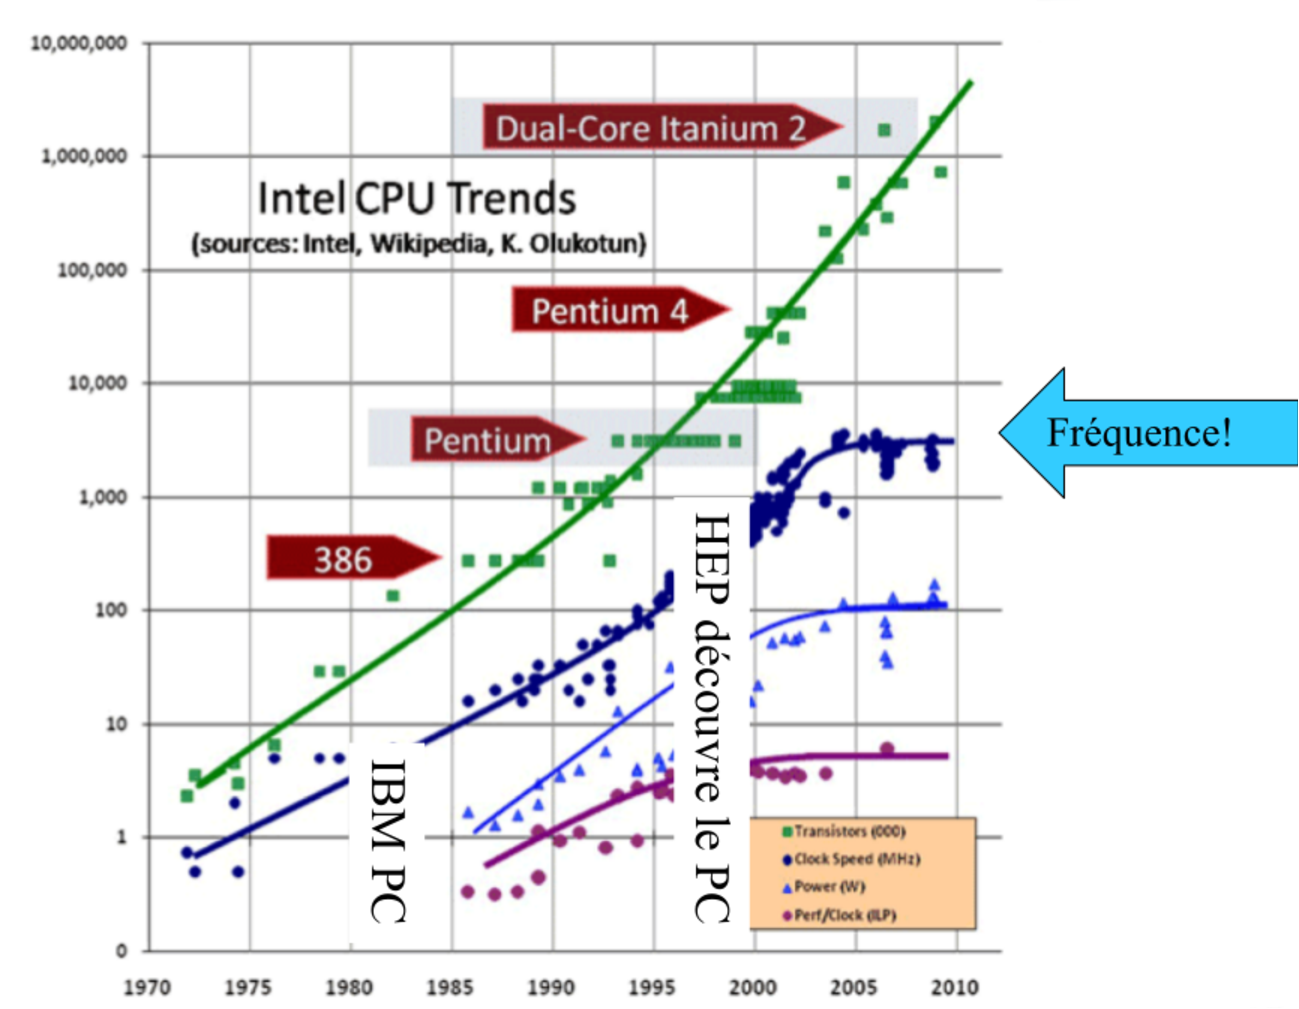
\includegraphics[width=0.85\textwidth]{figs/cpu-evol-freq.pdf}
  \end{center}
}

\frame{\frametitle{3 Walls: the free lunch is over}

  \begin{block}{}
    \begin{itemize}
    \item Moore's law still observed at the hardware level
    \item \myred{However} the \emph{``effective''} perceived computing
      power is mitigated
    \end{itemize}
  \end{block}

  \begin{columns}
    \begin{column}{0.5\textwidth}
      Confronted with 3 walls:
      \begin{itemize}
      \item \emph{power wall}
      \item \emph{memory wall}
        \item \emph{instruction level parallelism (ILP) wall}
      \end{itemize}
    \end{column}
    \begin{column}{0.5\textwidth}
      \begin{center}
        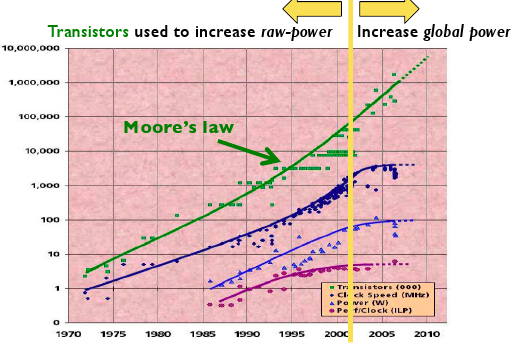
\includegraphics[width=0.99\textwidth]{figs/cpu-evol.png}
      \end{center}
    \end{column}
  \end{columns}
}

\frame{\frametitle{\emph{Power wall}}
  \emph{``Easy life''} during the last 20-30 years:
  \begin{itemize}
    \item \myred{Moore's law} translated into \myred{doubling} compute
      capacity every $\simeq 18$ months (\mypurple{clock frequency})
  \end{itemize}

  \myred{But issues with power dissipation}

  \begin{columns}

  \begin{column}{0.65\textwidth}
    \begin{block}{}
    Moore's law still observed at the hardware level:
    \begin{itemize}
      \item $\uparrow$ transitors $\Rightarrow$ $\uparrow$ number of
        cores
      \item keep clock frequency constant to limit energy consumption
    \end{itemize}
    \end{block}

    \begin{alertblock}{}
      \begin{center}
      \myred{Concurrency \& Parallelism} are necessary to efficiently
      harness the compute power of our new multi-cores \texttt{CPU}s
      architectures.
      \end{center}
    \end{alertblock}
  \end{column}

  \begin{column}{0.4\textwidth}
  \begin{center}
    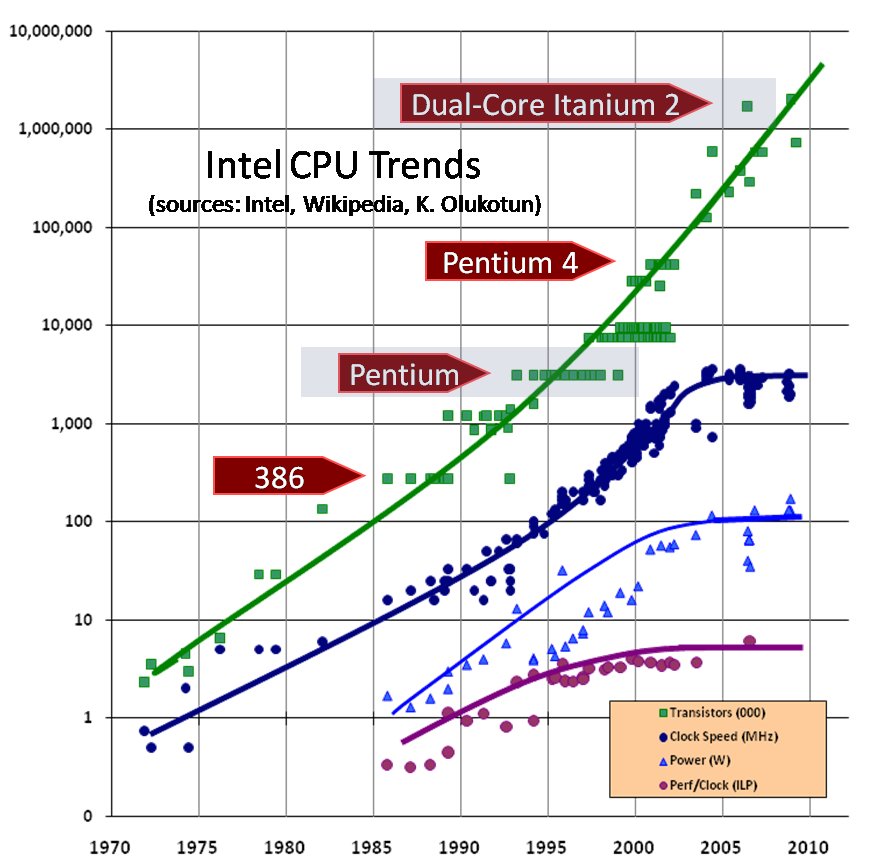
\includegraphics[width=0.99\textwidth]{figs/cpu-free-lunch.png}
  \end{center}
  \end{column}
  \end{columns}
}

\frame{
  \frametitle{\emph{Memory wall}}

  \begin{columns}
    \begin{column}{0.65\textwidth}
      \begin{itemize}
      \item clock frequency increases faster than memory
      \item bigger and faster caches somewhat mitigated impact (for
        now)
      \item memory access latency: \myred{bottleneck}
      \item introduce multi-level (hierarchical) memory caches
        \begin{itemize}
          \item for Intel Ivy Bridge (@3.4 $GHz$)
        \item \emph{L1}: $\sim 4 cycles$
        \item \emph{L2}: $\sim 12 cycles$
        \item \emph{L3}: $\sim 30 cycles$
        \item \emph{RAM}: $\sim 30 cycles + \sim 50ns$
        \end{itemize}
      \end{itemize}
  \end{column}

  \begin{column}{0.4\textwidth}
  \begin{center}
    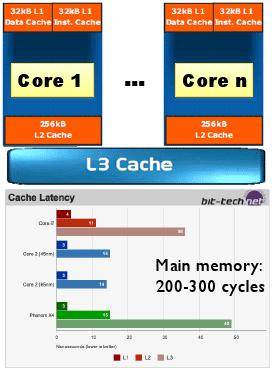
\includegraphics[width=0.99\textwidth]{figs/memory-wall.jpeg}
  \end{center}
  \end{column}
  \end{columns}
}

\frame{
  \frametitle{\emph{Architecture wall}}

  \begin{columns}
    \begin{column}{0.65\textwidth}
      \begin{itemize}
      \item pipelines deep and large
        \item various techniques to improve \mypurple{\emph{Instruction Level
          Parallelism}} (\texttt{ILP}):
          \begin{itemize}
          \item hardware branch prediction,
          \item hardware speculative execution,
          \item instruction re-ordering,
          \item \emph{Just-In-Time} (JIT) compilation,
          \item hardware threading, \ldots
          \end{itemize}

        \item in practice: inter-dependence issues between
          instructions \myred{limit application} of \texttt{ILP}
      \end{itemize}
  \end{column}

  \begin{column}{0.4\textwidth}
  \begin{center}
    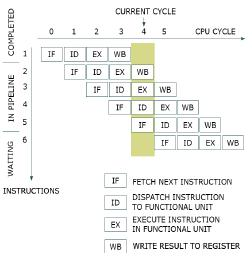
\includegraphics[width=0.99\textwidth]{figs/ilp-wall.jpeg}
  \end{center}
  \end{column}
  \end{columns}
}

\frame{
  \frametitle{3 walls: \emph{the free lunch is over}}
  \begin{center}
    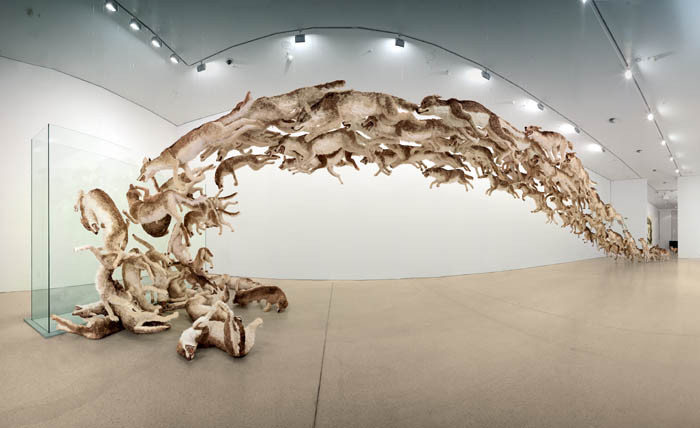
\includegraphics[width=0.99\textwidth]{figs/head-on.png}
  \end{center}
}


\begin{frame}
\frametitle{Pentium days}
\begin{columns}
  \begin{column}{0.5\textwidth}

    \begin{itemize}
    \item \alert{2} dimensions:
      \begin{itemize}
      \item \emph{pipeline} frequency
      \item number of nodes
      \end{itemize}
    \item semiconductor vendors were \alert{increasing frequency}
    \item users were buying adequate number of nodes
    \end{itemize}
  \end{column}
  \begin{column}{0.5\textwidth}
    
    \begin{center}
      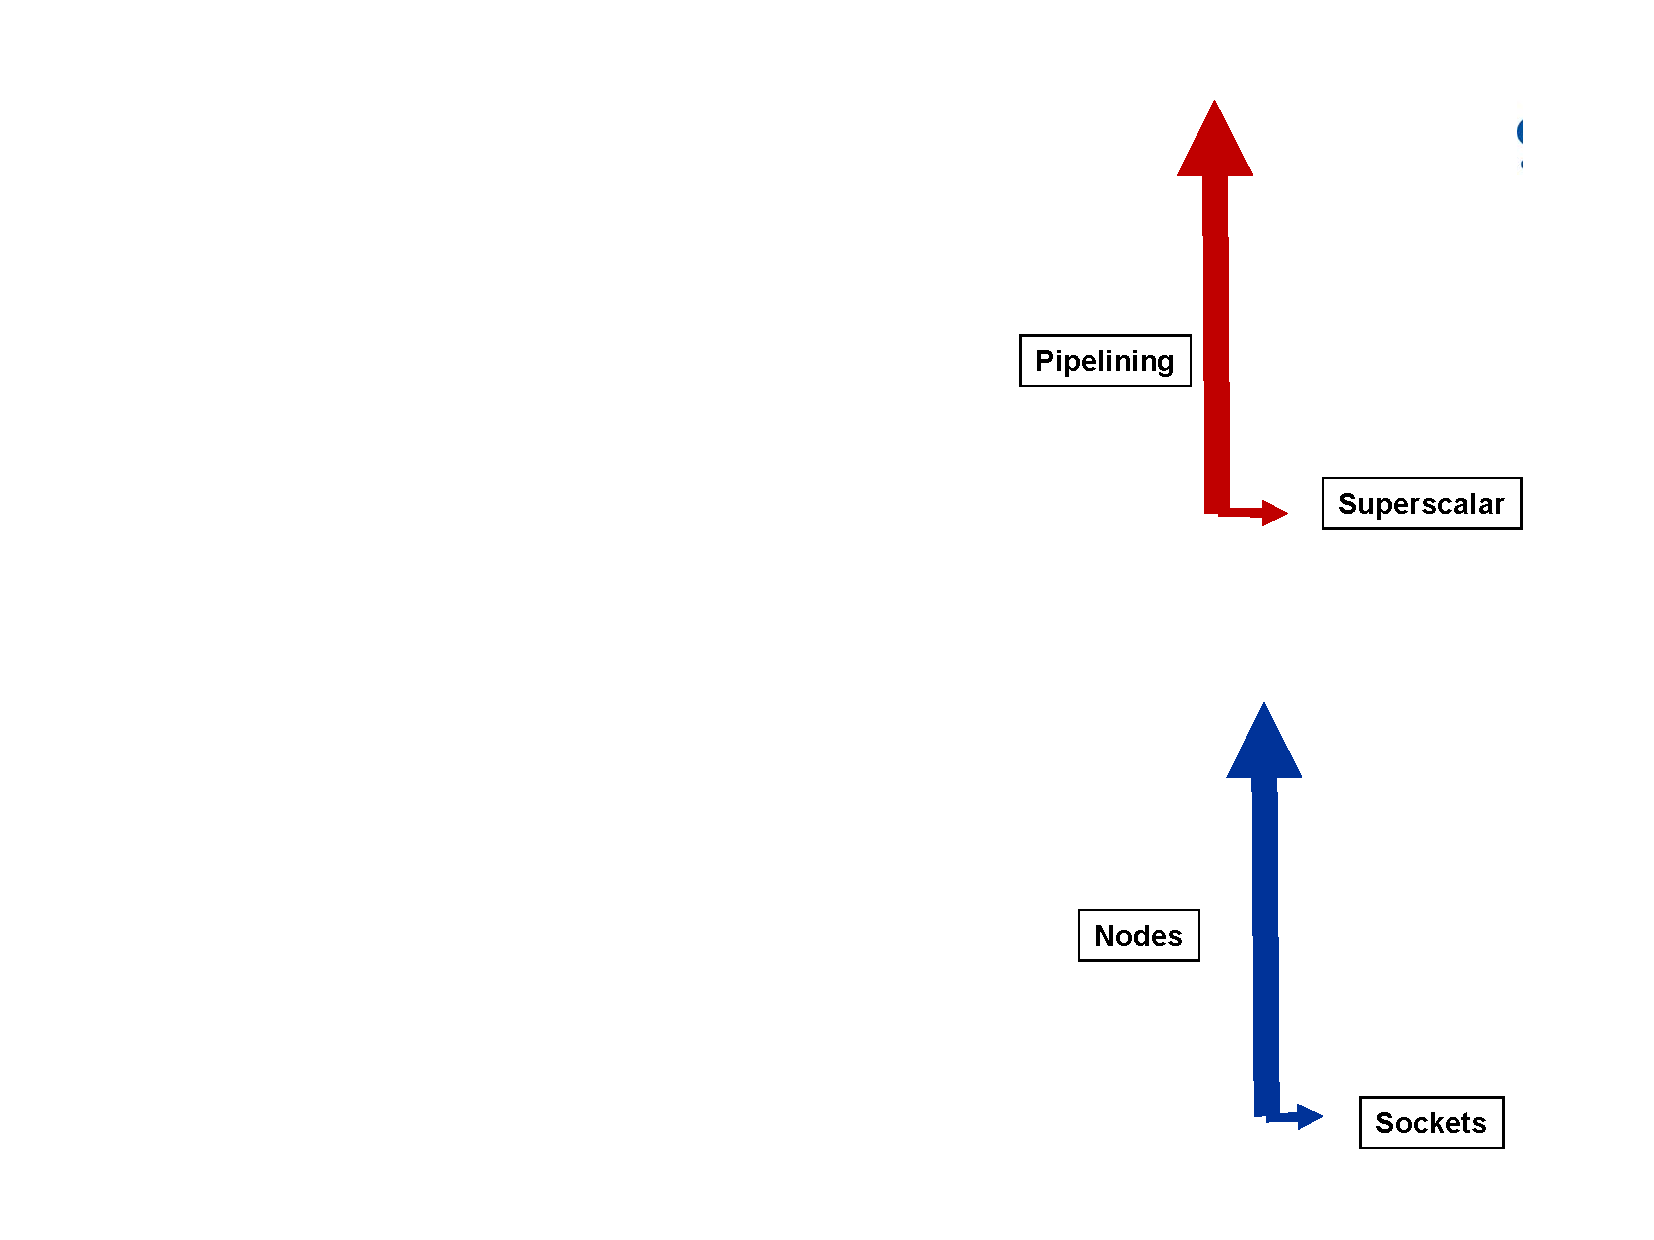
\includegraphics[width=.6\textwidth]{figs/sverre-pentium.pdf}
    \end{center}
  \end{column}
\end{columns}
\end{frame}

\begin{frame}
  \frametitle{Now: 7 dimensions}
  \begin{columns}
    \begin{column}{0.5\textwidth}

      \begin{itemize}
      \item first \alert{3} dimensions:
        \begin{itemize}
        \item vector units/\texttt{SIMD} (Single Instruction, Multiple Data)
        \item \emph{pipeline}
        \item \emph{superscalar}
        \end{itemize}
      \item ``pseudo'' dimension:
        \begin{itemize}
        \item hardware \emph{multithreading}
        \end{itemize}
      \item last \alert{3} dimensions:
        \begin{itemize}
        \item multi-cores
        \item multi-sockets
        \item multi-nodes
        \end{itemize}
      \end{itemize}
    \end{column}

    \begin{column}{0.5\textwidth}
      \begin{center}
        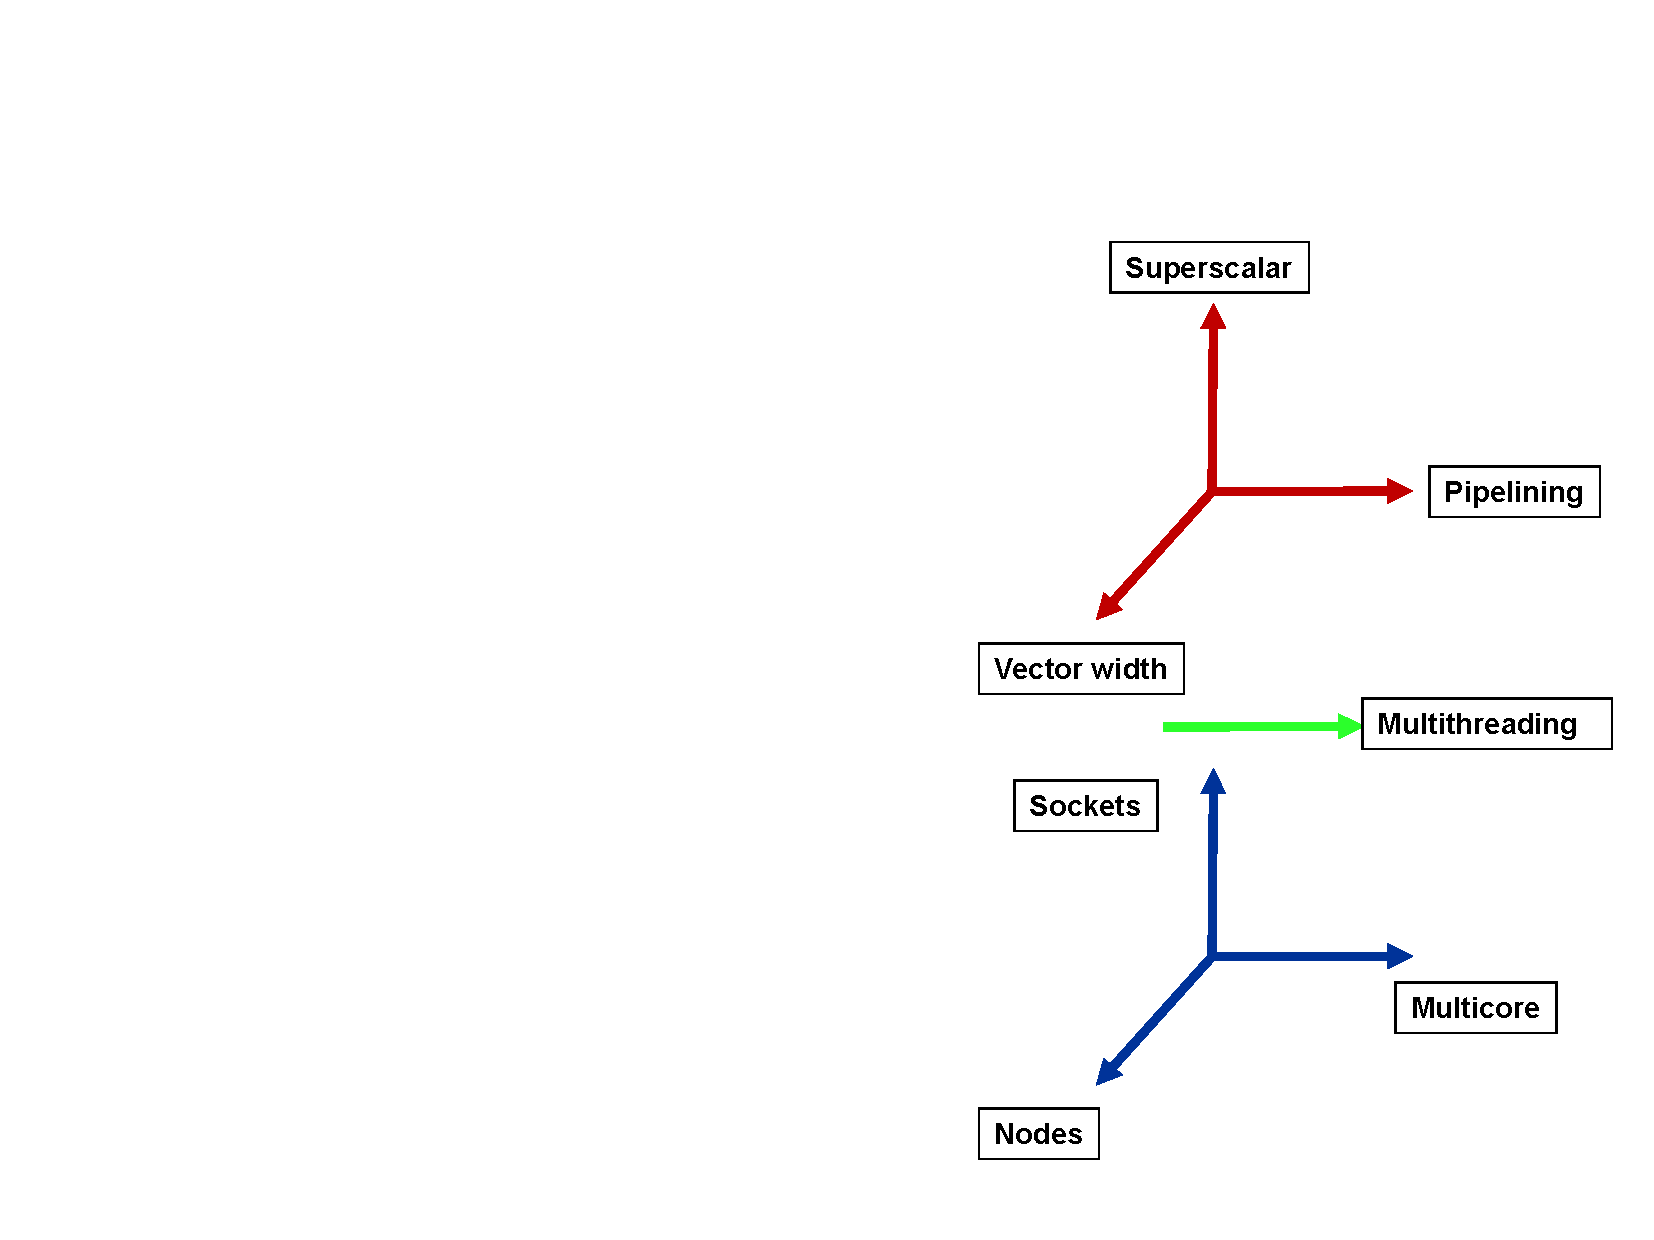
\includegraphics[width=.925\textwidth]{figs/sverre-seven-dims.pdf}
      \end{center}
    \end{column}
  \end{columns}
\end{frame}

\begin{frame}
  \frametitle{Now: 7 \emph{multiplicative} dimensions}

  \begin{columns}
    \begin{column}{0.5\textwidth}

      \begin{itemize}
      \item \alert{3} first dimensions:
        \begin{itemize}
        \item vector units/\texttt{SIMD}
        \item \emph{pipeline}
        \item \emph{superscalar}
        \end{itemize}
      \item ``pseudo'' dimension:
        \begin{itemize}
        \item \emph{multithreading} hardware
        \end{itemize}
      \item \alert{3} last dimensions:
        \begin{itemize}
        \item multi-cores
        \item multi-sockets
        \item multi-nodes
        \end{itemize}
      \end{itemize}
    \end{column}

    \begin{column}{0.5\textwidth}
      \begin{block}{Data-parallel}

        vectors/matrices
      \end{block}
      \begin{block}{Task-parallel}
        \begin{itemize}
        \item events
        \item tracks
        \end{itemize}
      \end{block}
      \begin{block}{Tasks/process-parallel}
      \end{block}
    \end{column}
  \end{columns}
\end{frame}

\begin{frame}
  \frametitle{Where are we now ?}

  \begin{center}
    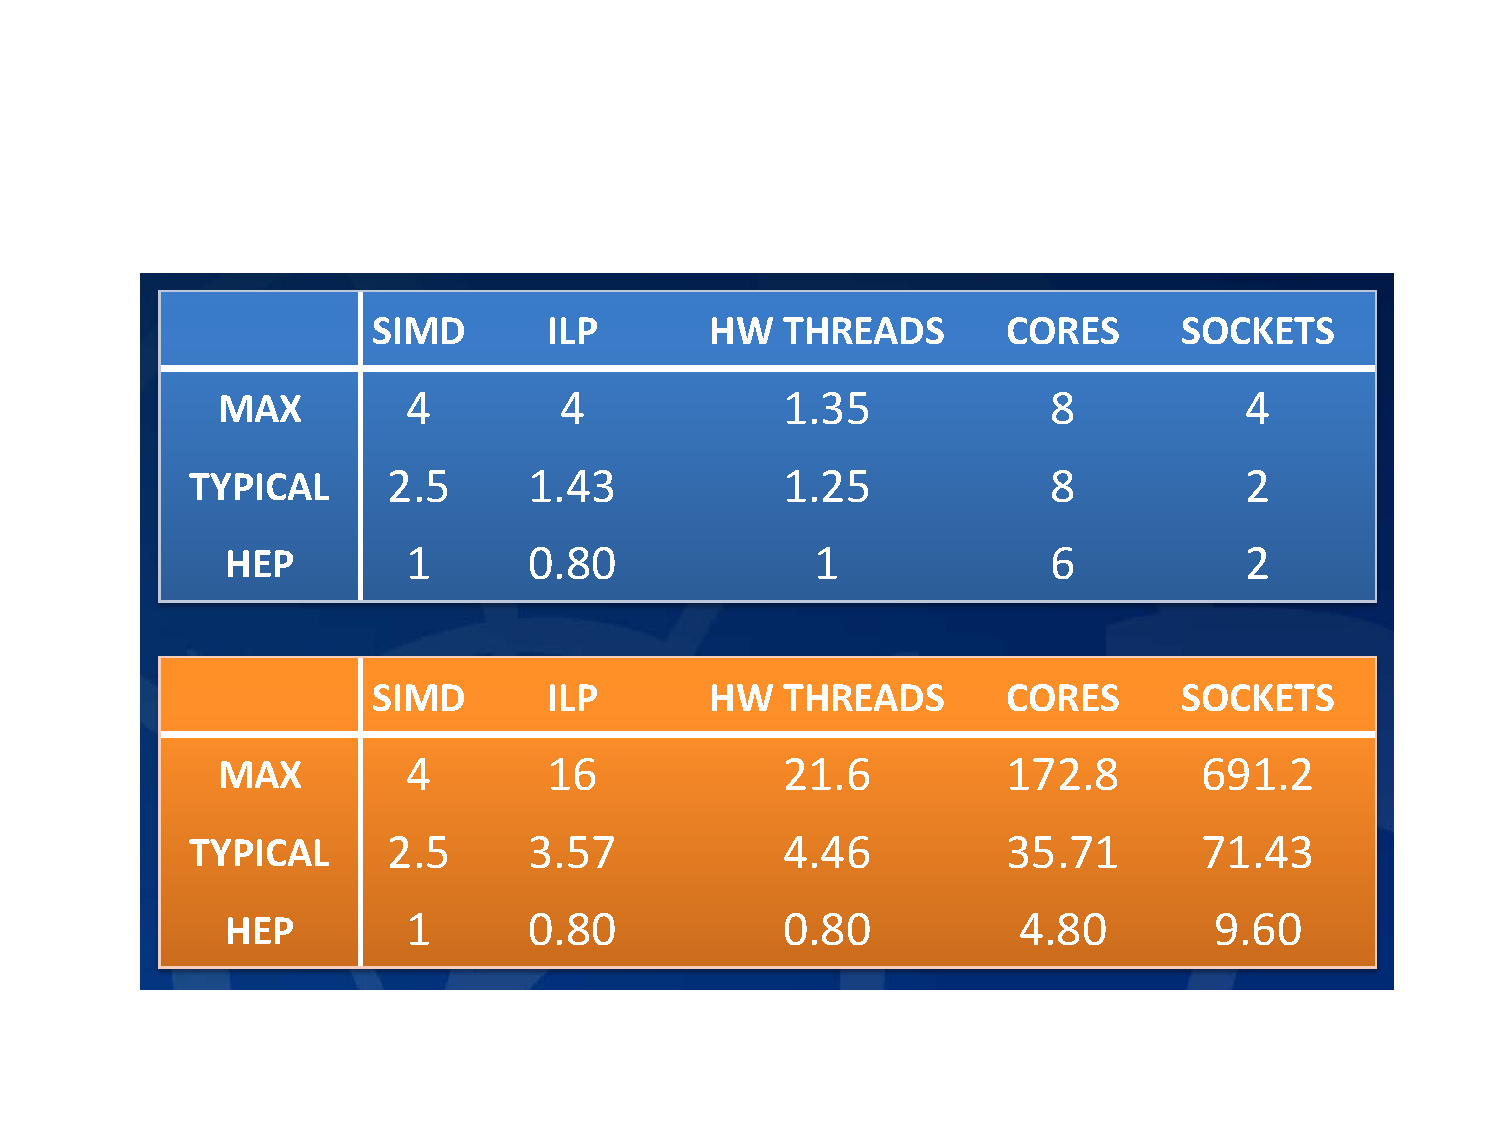
\includegraphics[width=1.\textwidth]{figs/nowak-ilp-cores.pdf}
  \end{center}

  A. Nowak (CERN/OpenLab)
\end{frame}

\begin{frame}
  \frametitle{Where do we go ? (dunno!)}


  \begin{center}
    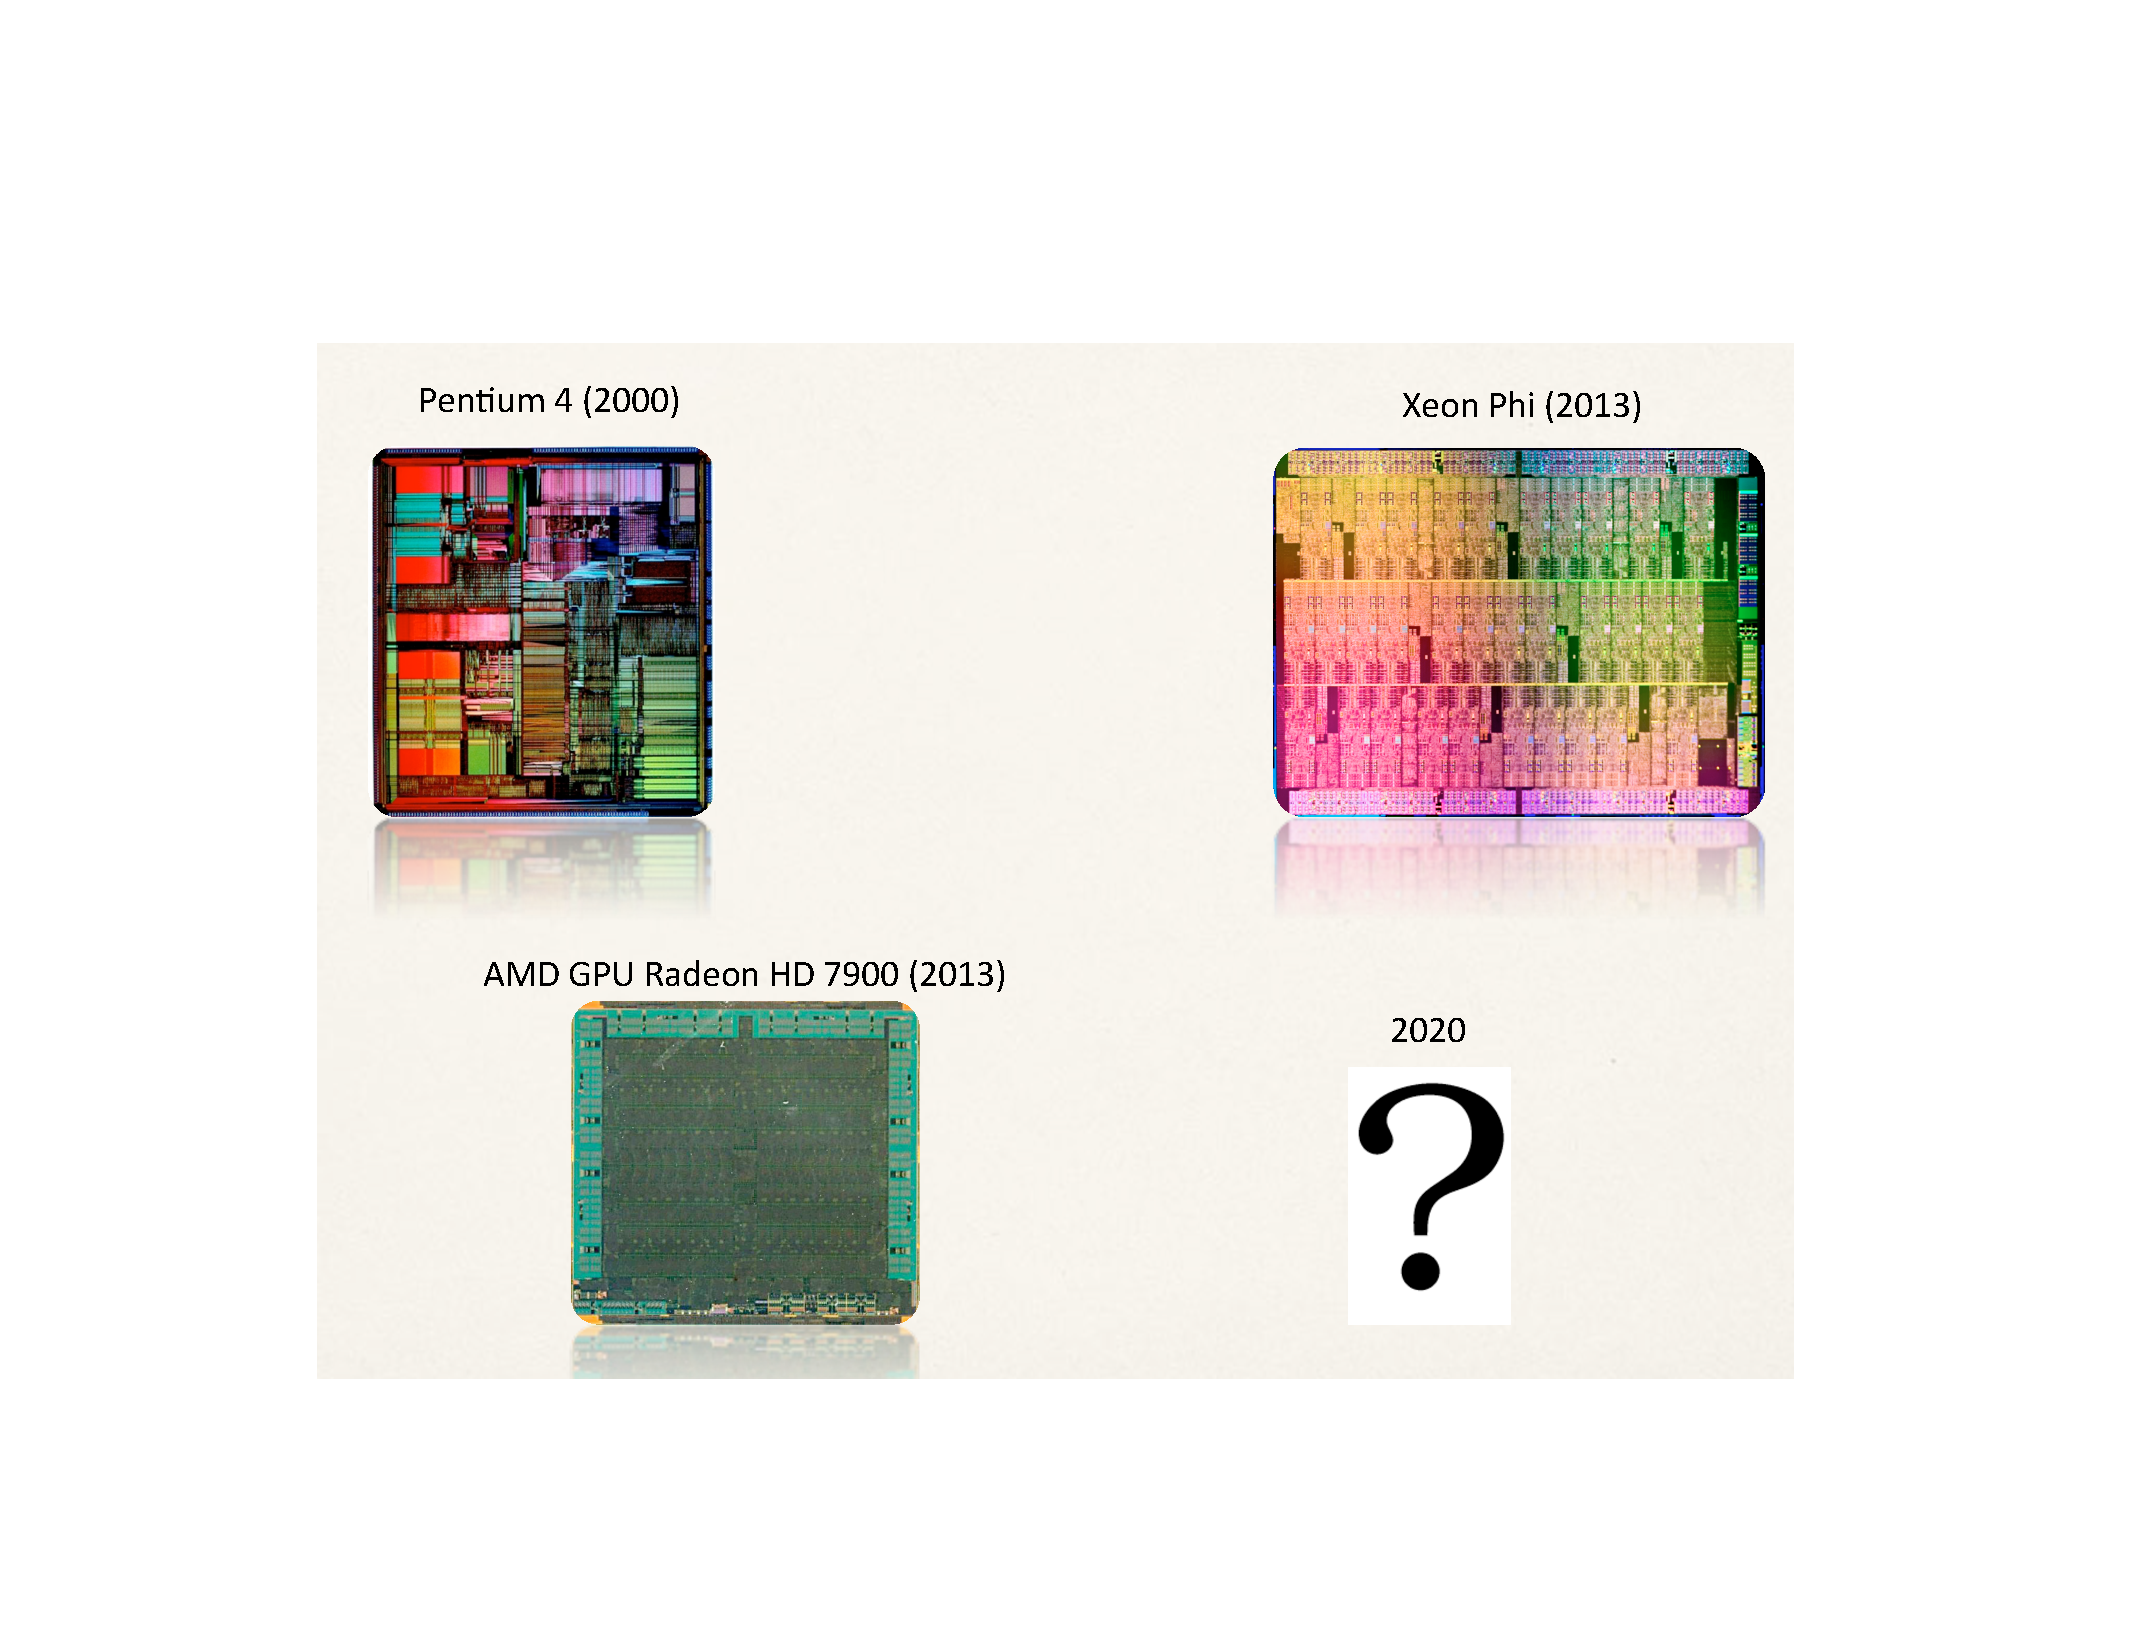
\includegraphics[width=1.\textwidth]{figs/pere-arch-cpus.pdf}
  \end{center}
\end{frame}

\begin{frame}
  \frametitle{Impact on HEP \emph{software}}

  \begin{block}{}
    \emph{CPU} $\Rightarrow$ multi-cores
    \begin{itemize}
    \item each \emph{CPU} may hold \alert{multiple} (2 $\rightarrow \sim$ 64) \alert{cores}
    \item each core is \alert{individually slower} than the ``old'' \emph{CPUs}
    \item available memory per core \alert{decreases}
    \end{itemize}
  \end{block}
  
  \begin{block}{}
   $\uparrow$ \emph{number of CPU} cores $\Rightarrow$ $\uparrow$ \alert{concurrency + parallelism}
    
    \begin{itemize}
    \item analysis \& reconstruction applications:
      \begin{itemize}
      \item parallelism at event level
      \item \emph{embarassingly parallel}
      \end{itemize}
    \item parallelism at algorithm level
      \begin{itemize}
      \item potentially more scalable
      \item more difficult too (code \emph{redesign/rewrite})
      \end{itemize}
    \end{itemize}
  \end{block}
  
  \begin{block}{}
   Amdahl's law: $R_{speedup} = \frac{1}{(1-S)+\frac{S}{N_{CPU}}}$
   \\
   harness parallelism \emph{via}:
    \begin{itemize}
    \item \mypurple{multi-processing} (\emph{eg:} \texttt{AthenaMP, GaudiMP, CMSSW, \ldots})
    \item \mypurple{multi-threading} (\emph{eg:} \texttt{AthenaMT, GaudiHive,
      Geant4-MT, CMSSW, \ldots})
    \end{itemize}
  \end{block}

\end{frame}

\begin{frame}
  \frametitle{Multi-processing: naive implementation}

Launch \emph{n} instances of an application on a node with \emph{n} cores

\begin{itemize}
\item re-use pre-existing code
\item \emph{a priori} no required modification of pre-existing code
\item satisfactory \emph{scalability} with the number of cores
\end{itemize}

\begin{block}{Problem(s)}

\begin{itemize}
\item resources requirements increase with the number of processes
\item \alert{$\uparrow$ memory footprint}
\item other OS (limited) resources: \emph{file descriptors}, \emph{network sockets},
  \ldots{}
\item share resources (+optimisation) - \emph{eg} on DAQ clusters

  \begin{itemize}
  \item manage number of running applications
  \item nbr of network connections towards \emph{readout} system
  \item transfer exact same configuration data \emph{n} times to same node
  \item recompute \emph{n} times exact same configuration data
  \item \emph{CPU} optimisation: interleave \emph{CPU} for event data handling and \emph{I/O-wait}
  \end{itemize}
\end{itemize}
\end{block}
\end{frame}

\begin{frame}
  \frametitle{Multiprocessing and memory sharing: \texttt{fork+COW}}
  \begin{block}{Principles}

    \begin{itemize}
    \item launch many similar jobs, sharing as much memory as possible
    \item minimize code modifications
      \begin{itemize}
      \item let the OS perform most of the work for us
      \end{itemize}
    \item use the \alert{\texttt{fork()}} system call
    \end{itemize}
  \end{block}

  \begin{block}{\texttt{fork()}}

    \begin{itemize}
    \item \texttt{fork()} clones a process, including its entire address space
    \item \texttt{fork()}, on modern OSes, is implemented via \alert{Copy On Write (COW)}
      \begin{itemize}
      \item all the memory pages are shared until a process writes on them
      \item these memory pages are then copied and become un-shared
      \end{itemize}
    \item $\Rightarrow$ \texttt{fork()} as late as possible \alert{but before} disk I/O
    \item \alert{optimal and AUTOMATED sharing} of the memory between sub-processes
      \begin{itemize}
      \item coupled to an OS + kernel version \ldots{}
      \item isolation between sub-processes
      \item \emph{Chromium and Firefox} use this technique (\texttt{Zygote process})
      \end{itemize}
    \end{itemize}
  \end{block}
\end{frame}

\begin{frame}
\frametitle{Multiprocessing and memory sharing: \texttt{fork+COW}}
\begin{block}{}
\begin{itemize}
  \item pros:
    \begin{itemize}
      \item \mypurple{ALL} the memory that can be share \mypurple{will be shared}
      \item modifications restricted to a few \emph{core framework packages}
      \item no need for \mygreen{locks/mutexes}
    \end{itemize}
\end{itemize}
\end{block}

\begin{exampleblock}{}
  \begin{itemize}
    \item cons
      \begin{itemize}
        \item once \emph{un-shared}, memory can not be \mypurple{re-shared}
          \begin{itemize}
            \item issue for \emph{conditions data}
          \end{itemize}
      \end{itemize}
  \end{itemize}
\end{exampleblock}

\begin{figure}
  \begin{center}
    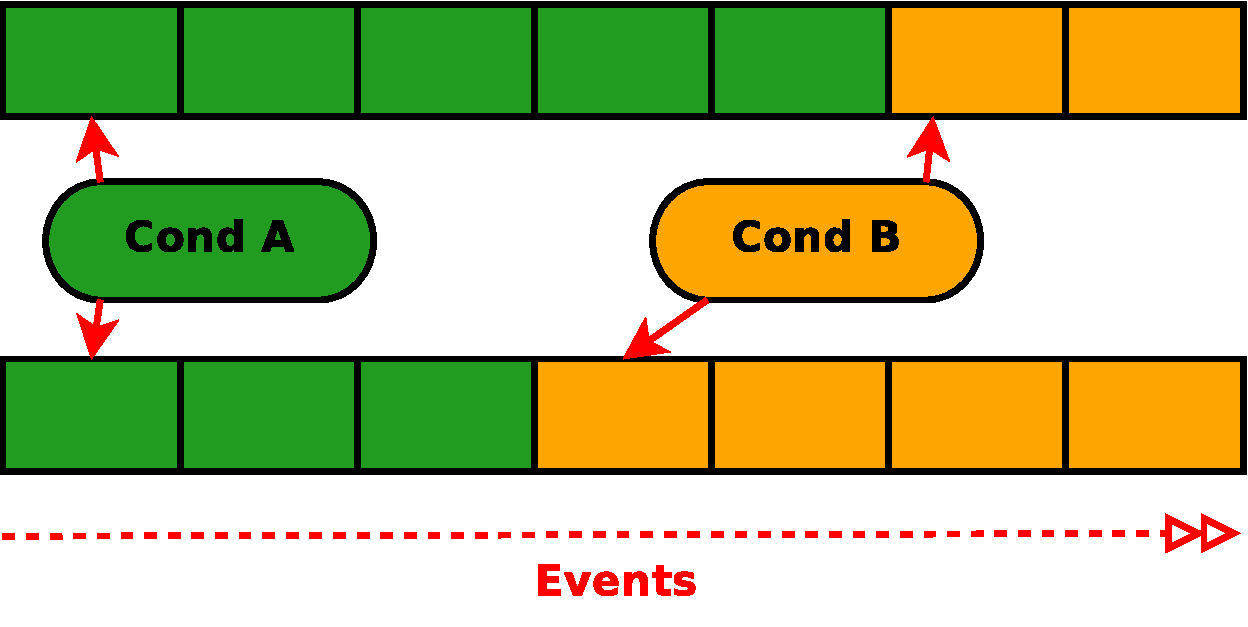
\includegraphics[angle=0,width=0.65\textwidth]{figs/cond-data-flow.pdf}
  \end{center}
\end{figure}
\end{frame}

\begin{frame}
\frametitle{Example: \texttt{AthenaMP} (\textsc{Atlas} reconstruction)}

  \begin{columns}
    \begin{column}{0.95\textwidth}

      \begin{block}{}
        \begin{itemize}
          \item minimize impact on client/physicist code
          \item use a \texttt{python} module \mygreen{\texttt{multiprocessing}} for process' management
          \begin{itemize}
            \item now re-written in \texttt{C++} (\texttt{AthenaMP-2})
          \end{itemize}
        \item encapsulate modifications related to parallelism inside a new event loop scheduler.
        \item modifications of \texttt{I/O}-related components
        \end{itemize}
      \end{block}

    \end{column}
  \end{columns}

  \begin{figure}
    \begin{center}
      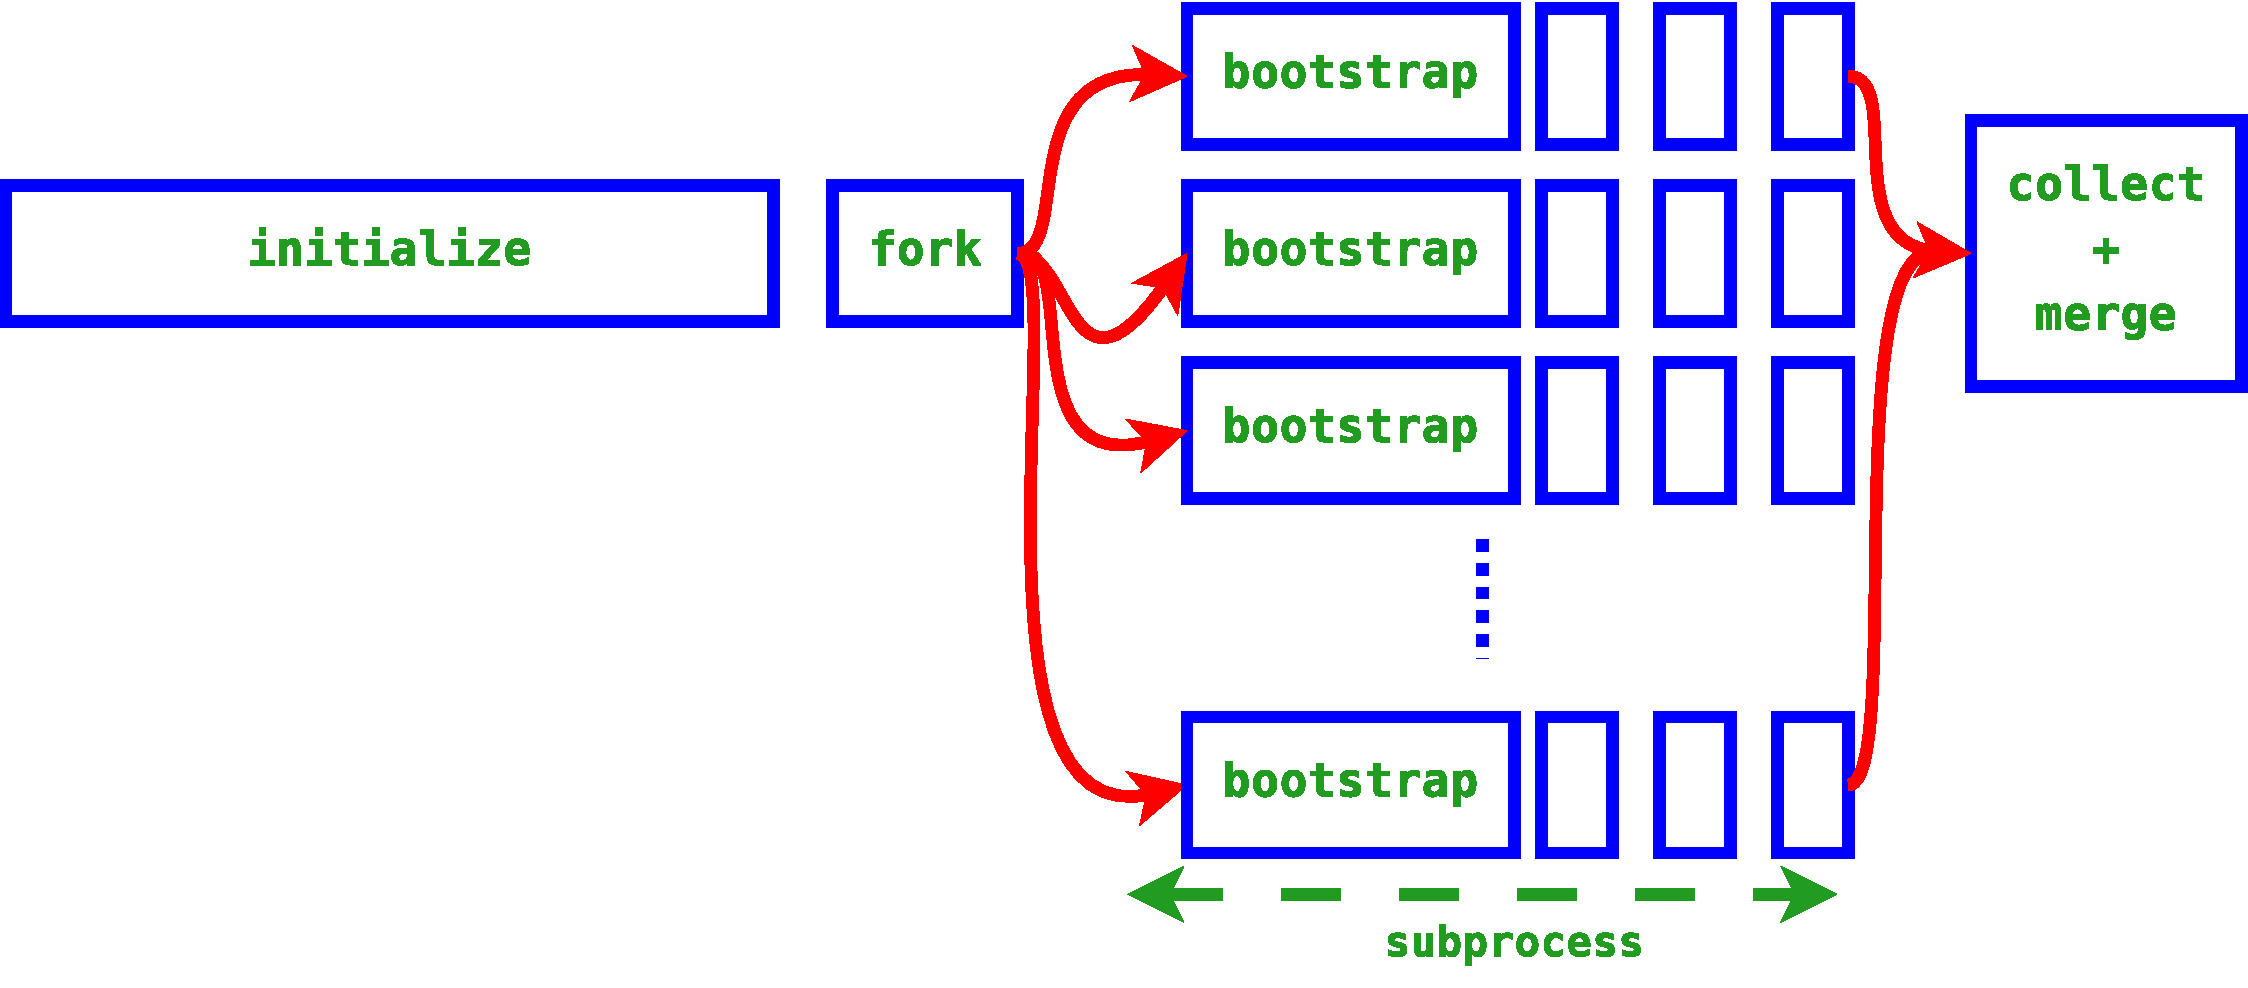
\includegraphics[angle=0,width=0.8\textwidth]{figs/athenamp-sequence.pdf}
    \end{center}
  \end{figure}
\end{frame}

\begin{frame}
\begin{columns}
\begin{column}{0.6\textwidth}

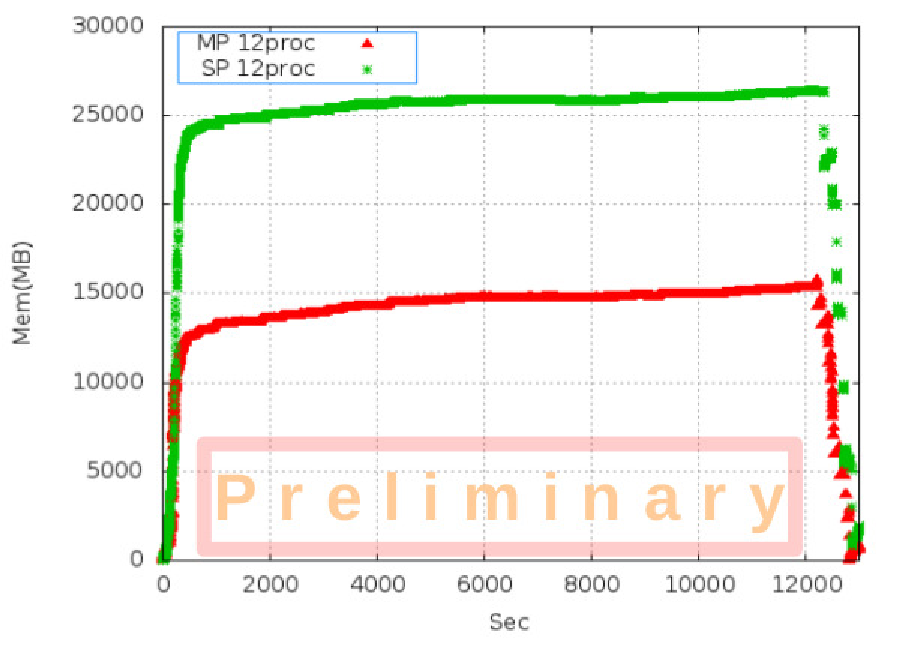
\includegraphics[width=.9\linewidth]{figs/athenamp-mem-savings.pdf}
\end{column}
\begin{column}{0.5\textwidth}

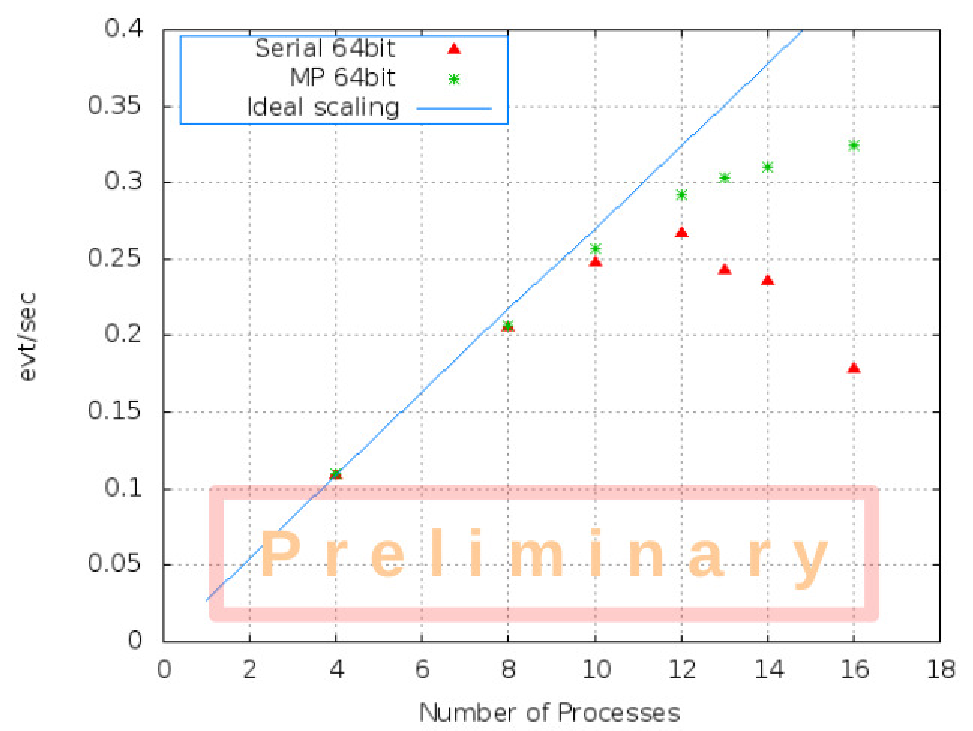
\includegraphics[width=.9\linewidth]{figs/athenamp-throughput-savings.pdf}
\end{column}
\end{columns}

\begin{itemize}
\item SP: \emph{n} \texttt{Athena} in parallel ($\Rightarrow$ $\sim$ 2Gb per proc.)
\item MP: \texttt{AthenaMP} ($\Rightarrow$ $\sim$ 1.2Gb per process)
\begin{itemize}
\item \alert{allow to do more physics with the same h/w}
\end{itemize}
\end{itemize}
\end{frame}

\frame{
  \frametitle{Experiences with multi-processes}
\begin{block}{}
  \begin{itemize}
    \item limited long range impact
    \item modifications applied to control framework and I/O-related components
    \item easier to develop with
      \begin{itemize}
        \item no implicit sharing
        \item no lock, races, \ldots
      \end{itemize}
  \end{itemize}
\end{block}

\begin{alertblock}{Problems}
  \begin{itemize}
    \item random numbers, seeds and reproducibility
    \item I/O
      \begin{itemize}
        \item need to chase people directly \texttt{open()}ing files, by-passing framework hooks
        \item merging output files is tedious (but needed for production)
      \end{itemize}
    \item GRID
      \begin{itemize}
        \item submission of MP-jobs (overbooking computing nodes)
        \item \texttt{vmem} accounting
          \begin{itemize}
            \item most of grid resource monitoring tools will double-count the memory shared by \texttt{fork()}ed subprocesses
          \end{itemize}
      \end{itemize}
  \end{itemize}
\end{alertblock}
}

\frame{
  \frametitle{(first) Conclusions}

\begin{exampleblock}{}
  \begin{center}
    It is possible to refactor an already existing
    \texttt{FORTRAN/C/C++} application, written in a
    \emph{single-threaded} fashion (like \texttt{Gaudi}) with minimal
    modifications (or at least \myred{localised}) to better leverage
    the \emph{new} multicore architectures.
  \end{center}
\end{exampleblock}

\begin{alertblock}{}
Automa(g)ic \emph{scaling} with the number of cores ?
\begin{itemize}
 \item unlikely if $N_{\texttt{cores}} \geq 1024$ (memory resources)
 \item unlikely at the \texttt{I/O} level
 \item \emph{mapping} 1 processus per core \myred{not fine-grained enough}
\end{itemize}
\end{alertblock}

\begin{block}{}
\begin{center}
 \begin{itemize}
  \item \myred{concurrency} at the \mypurple{event} level
  \item \myred{concurrency} at the \mypurple{algorithm} level
  \item \myred{concurrency} \mypurple{within the algorithms}
 \end{itemize}

$\Rightarrow$ \myred{multithreading !}\\
\end{center}
\end{block}
}

\frame{
  \frametitle{Interlude: Parallelism \& Concurrency}
  \begin{block}{}
  \begin{itemize}
    \item Concurrency is about \mypurple{dealing} with lots of things at once.
    \item Parallelism is about \mypurple{doing} lots of things at once.
    \item \myred{Not the same, but related.}
    \item Concurrency is about \mypurple{structure}, parallelism is about \mypurple{execution}.
    \item Concurrency provides a way to structure a solution to solve a
      problem that may (but not necessarily) be parallelizable.
  \end{itemize}
  \end{block}

  \begin{center}
    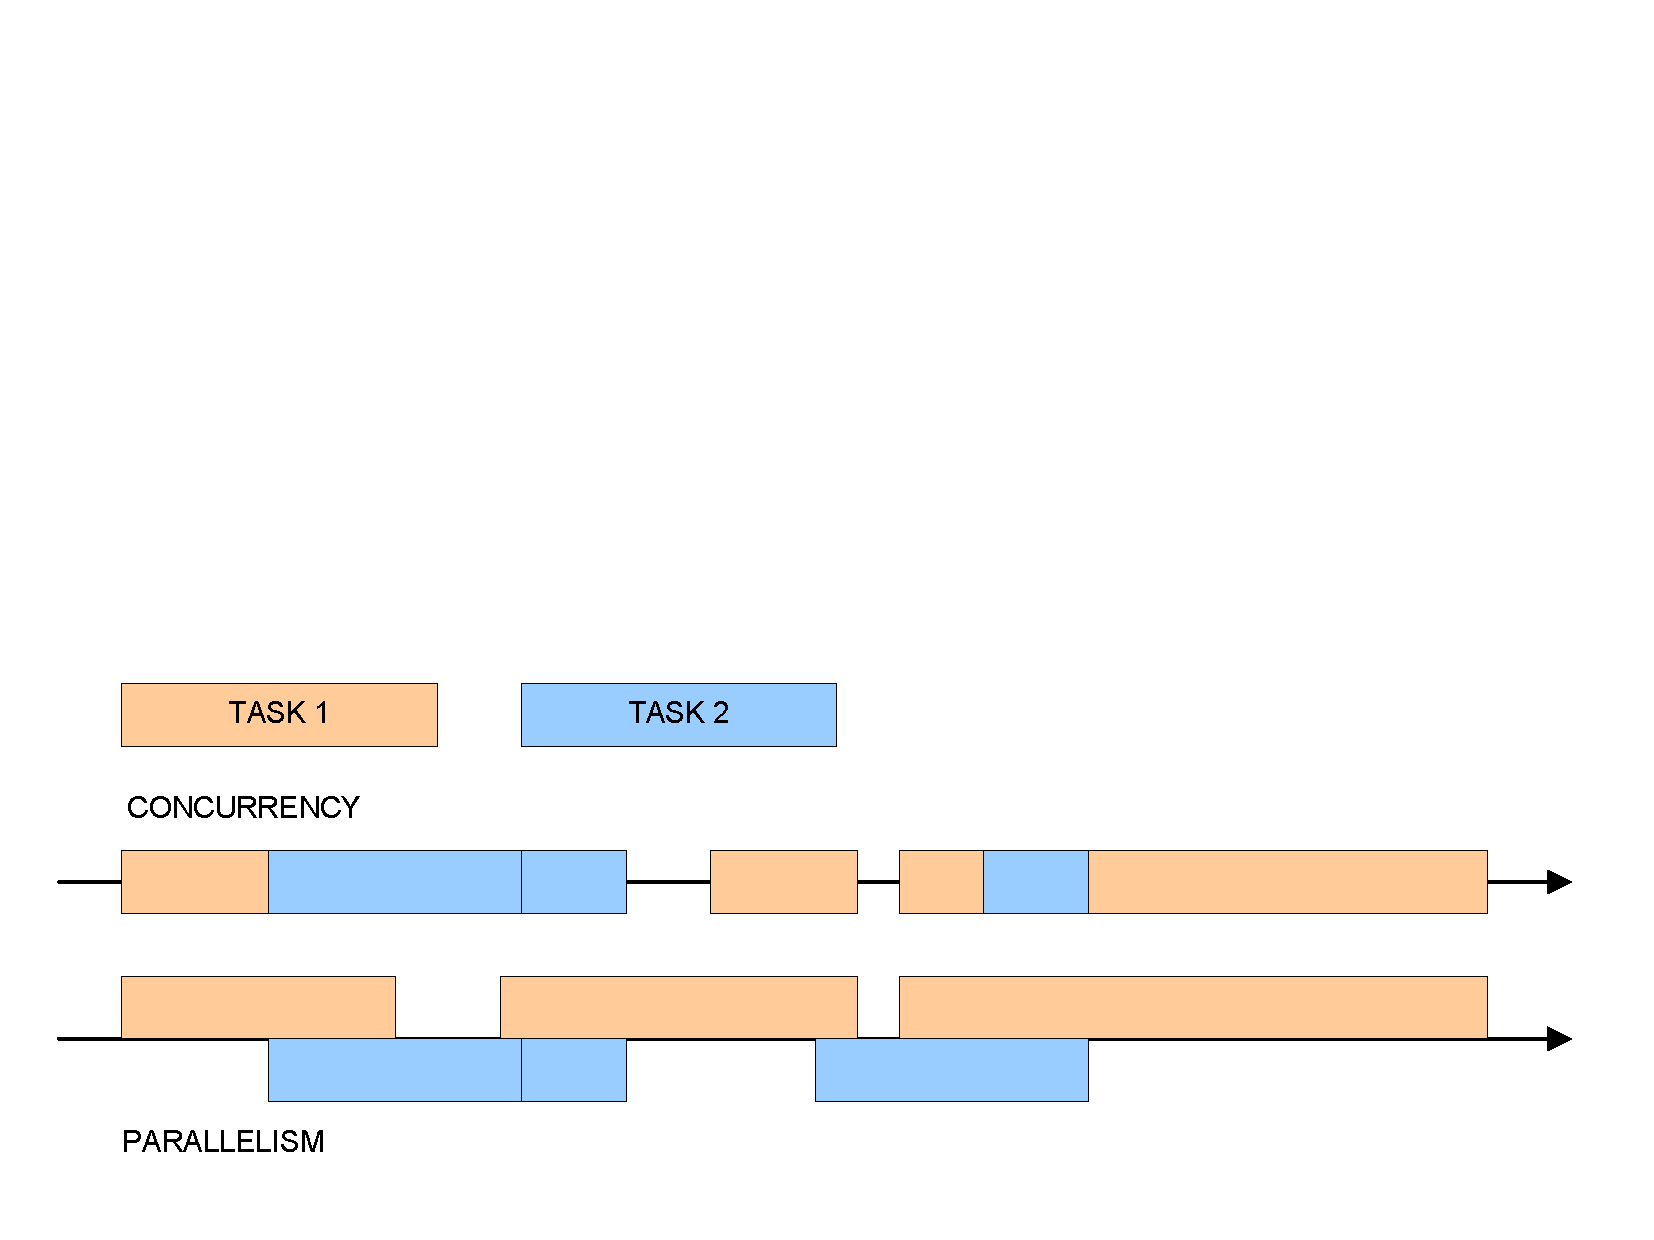
\includegraphics[width=0.65\textwidth]{figs/conc-para.pdf}
  \end{center}

  \begin{block}{Concurrency plus communication}
  Concurrency is a way to structure a program by breaking it into
  pieces that can be executed independently.
  Communication is the means to coordinate the independent executions.
  \end{block}

}


\frame{
  \frametitle{Concurrency in \verb~HEP~ frameworks}
New developments and/or adiabatic evolution of \texttt{Gaudi} need to:

\begin{itemize}
\item prepare for further \alert{gains} by exploiting features of today's CPUs' 
  $\mu$-architecture
\begin{itemize}
\item vector registers, instruction pipelining, multiple instructions per cycle
    (see Sverre Jarp presentations at CHEP)
\item improve data and code locality, hardware threading
\item (also relevant for non-fwk code)
\end{itemize}
\item prepare for, or at least don't prevent use of, 
  \alert{off-loading large computations} to accelerators (GPGPUS, Xeon Phi)
\item prepare for increased exposed concurrency
\begin{itemize}
\item a means for better memory usage and improved throughput
\end{itemize}
\end{itemize}
}

\frame{
\frametitle{Concurrency in \verb~HEP~ frameworks - II}
\begin{center}
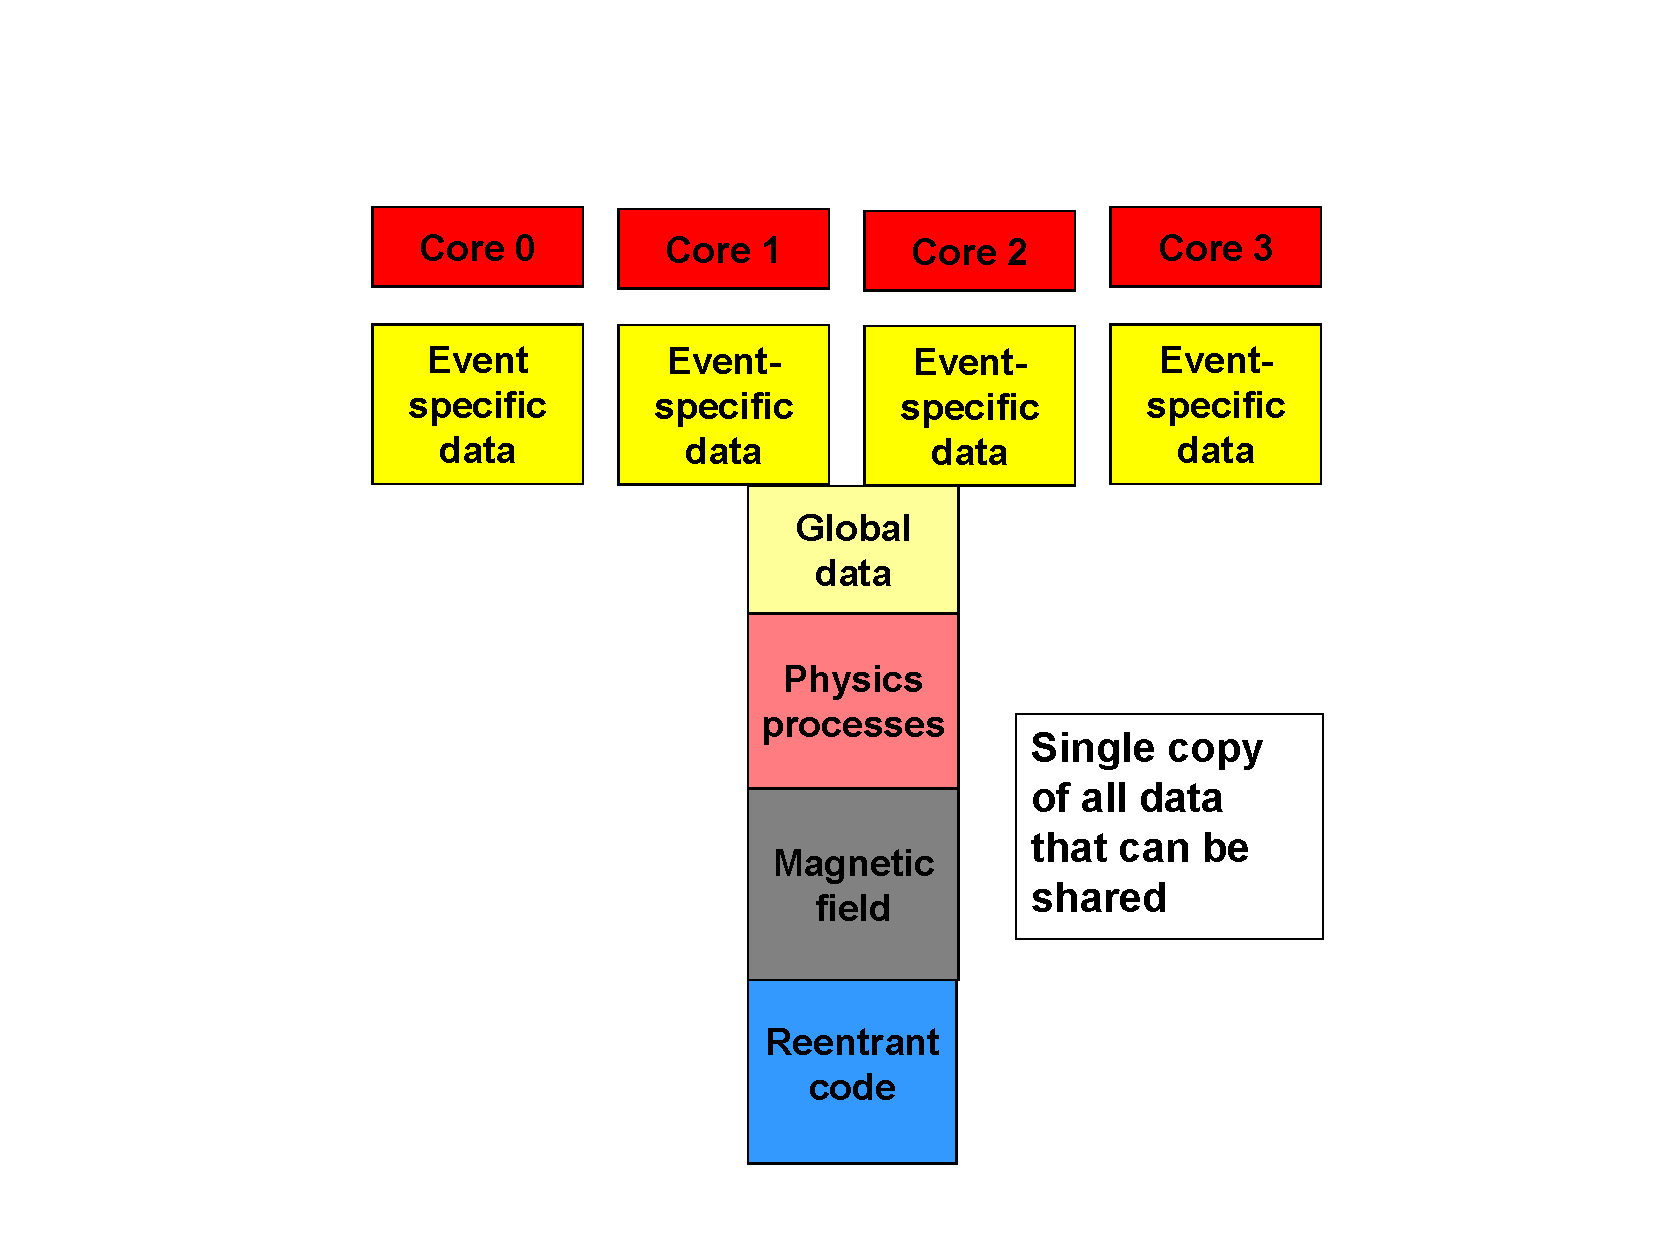
\includegraphics[width=0.66\linewidth]{figs/conc-level.pdf}
\end{center}
}

\begin{frame}[fragile]
\frametitle{Concurrency in \verb~HEP~ frameworks - III}


Various levels of concurrency can be exposed in current \verb~HEP~ applications:

\begin{itemize}
\item \alert{event-level} concurrency
\begin{itemize}
\item the framework allows to properly and safely process multiple events
    at a given time
\end{itemize}
\item \alert{algorithm-level} concurrency, \alert{task-} and/or \alert{data-} oriented concurrency
\begin{itemize}
\item the framework allows to partition the processing of an event into various
    sub-tasks (calorimetry, tracking, RoIs, \ldots{})
\item \alert{task/functional} oriented concurrency: split according to ``logical'' tasks
\item \alert{data} oriented concurrency: partition the data domain
\end{itemize}
\item \alert{subalgorithm-level} concurrency
\begin{itemize}
\item each algorithm can itself exposes concurrent sub-sub-tasks
\item leverage co-processors, vector units, \ldots{}
\end{itemize}
\end{itemize}
\end{frame}

\begin{frame}[fragile]
\frametitle{Concurrency in \verb~HEP~ frameworks - IV}


\alert{Event-level} concurrency is achieved by:

\begin{itemize}
\item modifying the event loop to hand over multiple events
\item put these multiple events into multiple event stores
\item have algorithms and sequence of algorithms work on these stores
\end{itemize}

\alert{REQUIRES} that at least the core components are \alert{race-free} and \alert{thread-safe}
\end{frame}
\begin{frame}[fragile]
\frametitle{Concurrency in \verb~HEP~ frameworks - V}


\alert{Alg-level} concurrency is achieved by:

\begin{itemize}
\item modifying the algorithm manager to execute multiple algorithms concurrently
\item \alert{need} new information to properly schedule these algorithms in the correct
  order: \alert{data dependency graph} (hopefully acyclic!)
\begin{itemize}
\item either extracted at \alert{runtime} during a warm-up
    phase or \alert{explicitly} at \alert{configuration-time}
\end{itemize}
\end{itemize}

\begin{figure}
  \begin{center}
    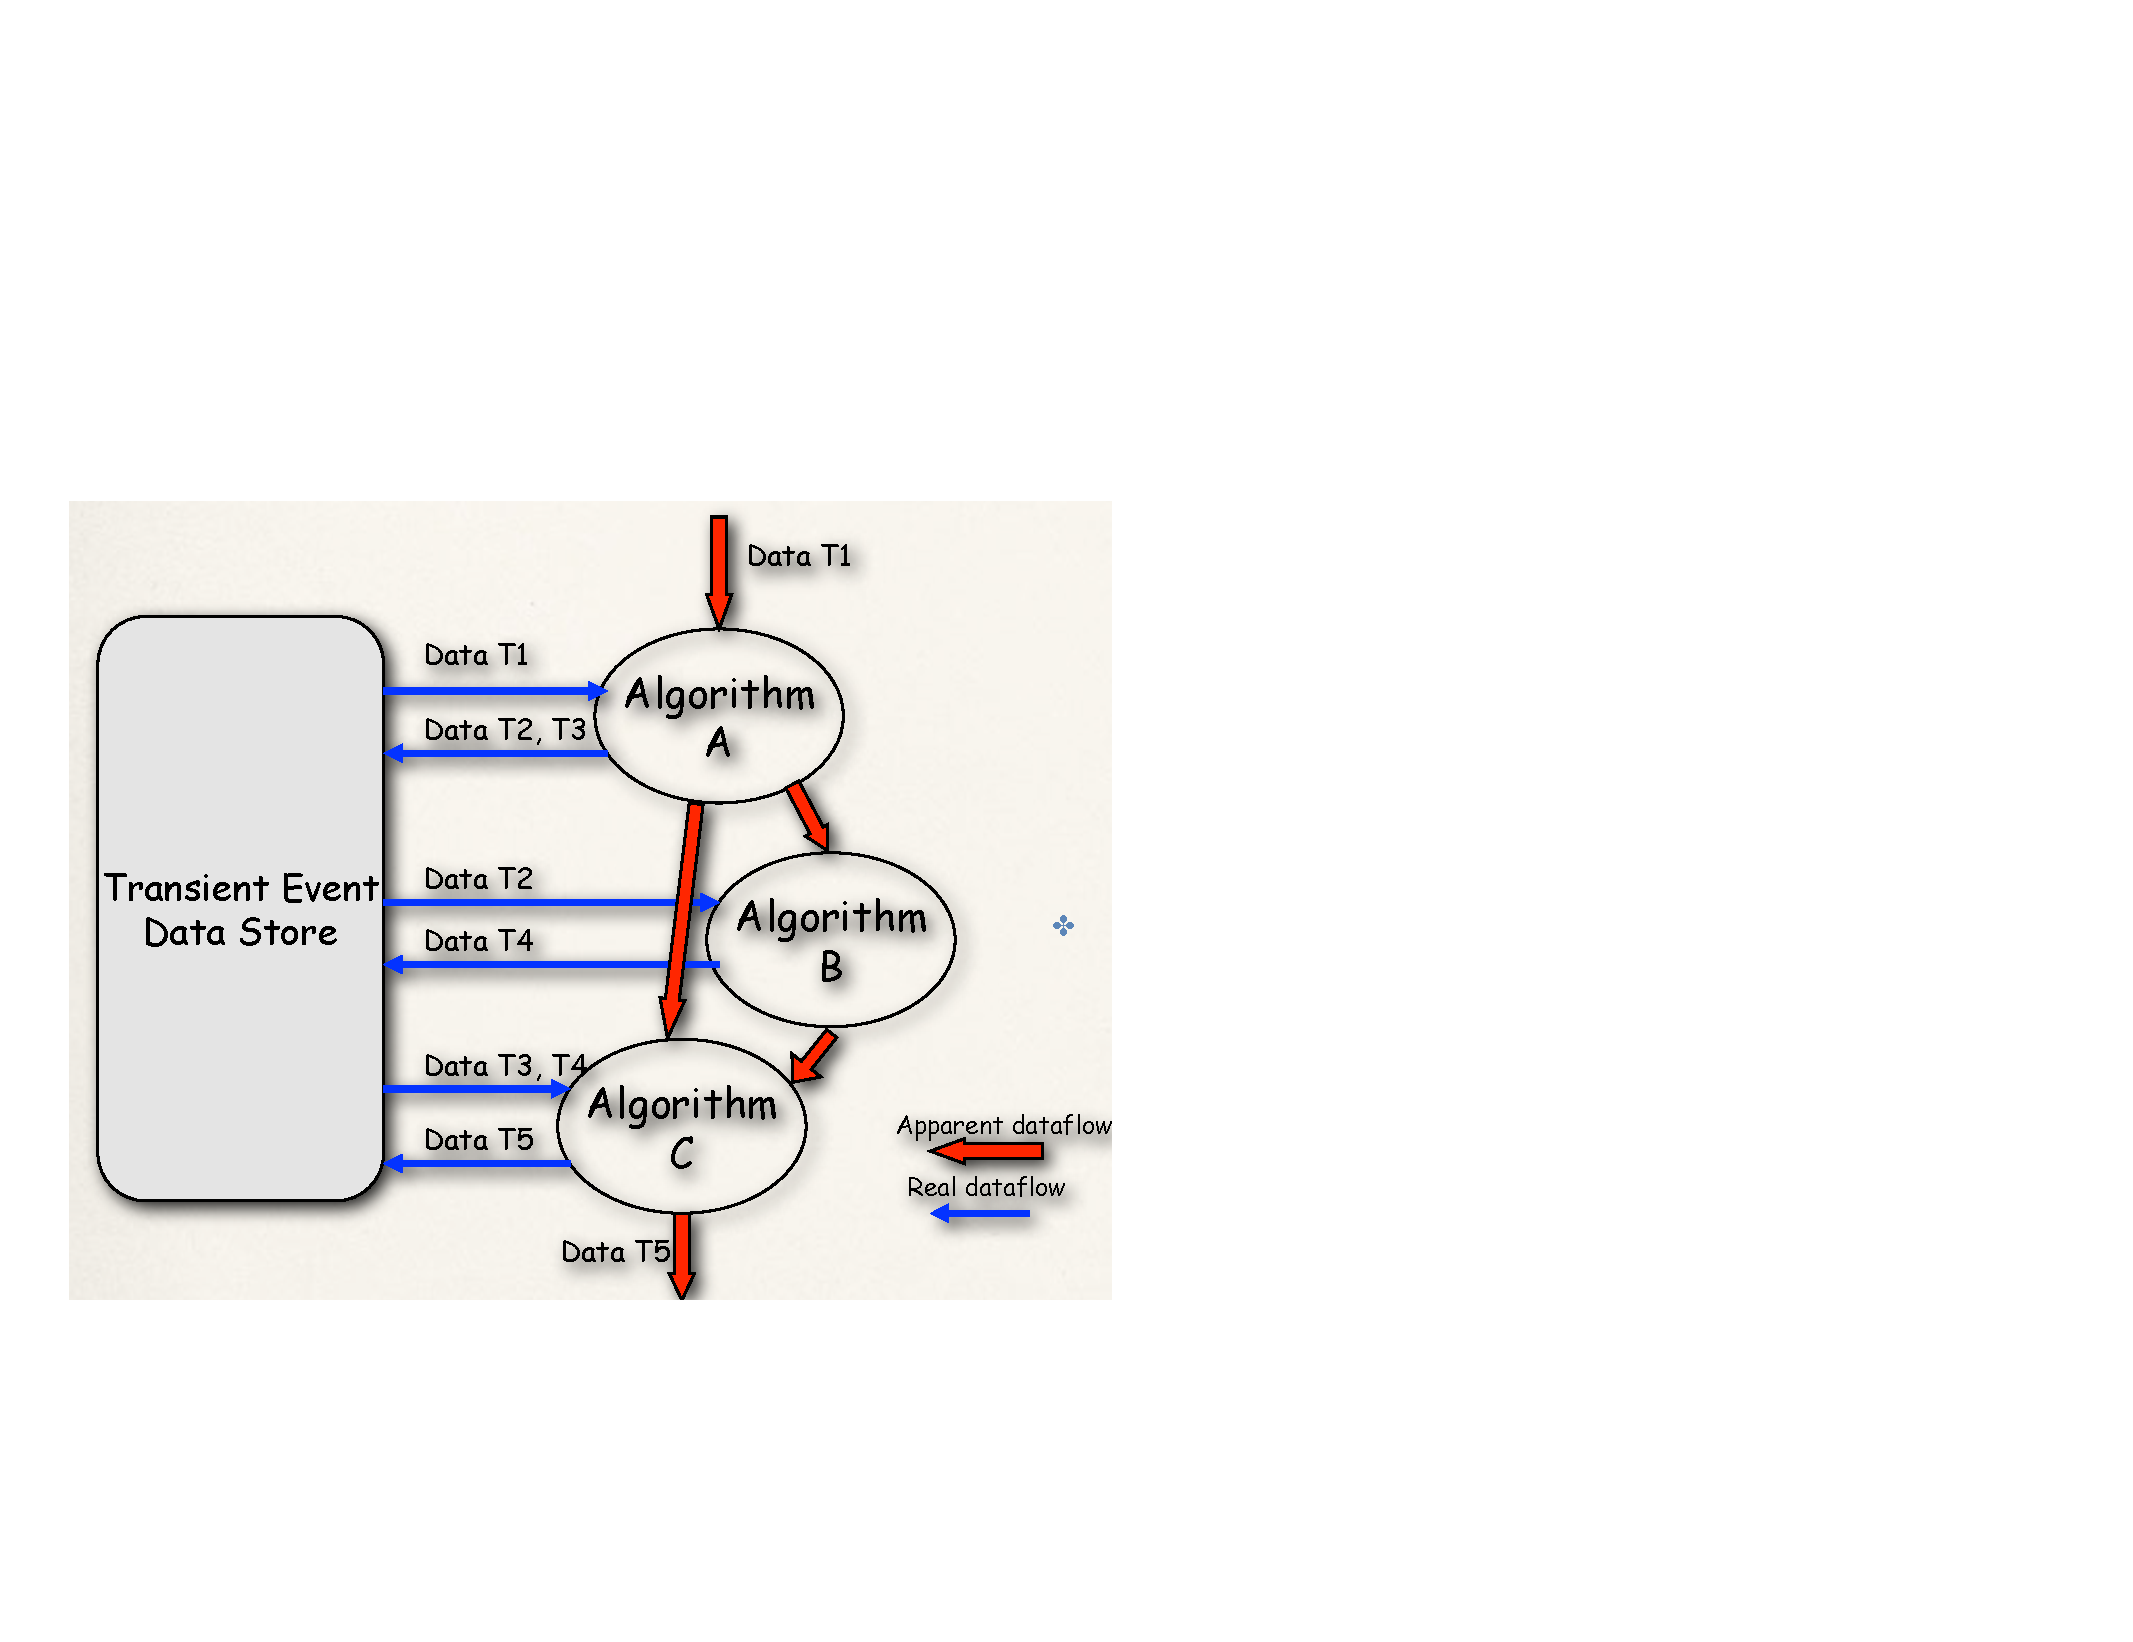
\includegraphics[width=0.45\textwidth]{figs/data-flow.pdf}
    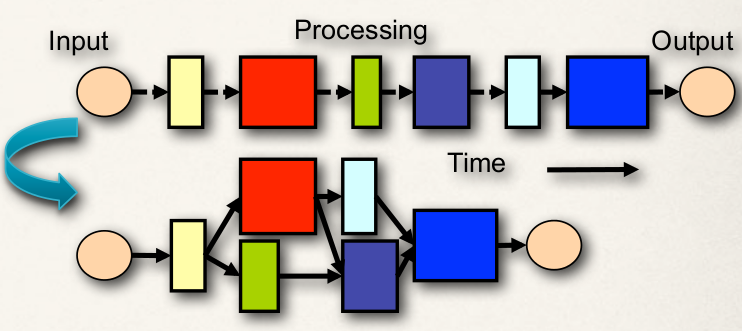
\includegraphics[width=0.45\textwidth]{figs/gaudi-hive-1.png}
  \end{center}
\end{figure}
\end{frame}
\begin{frame}[fragile]
\frametitle{Concurrency in \verb~HEP~ frameworks - VI}


\alert{SubAlg-level} concurrency is achieved by:

\begin{itemize}
\item providing tools or libraries to expose concurrency
\item making the framework aware of the available resources
\item making the framework aware of the different tools/libraries for
  an efficient scheduling
\end{itemize}
\end{frame}

\frame{
  \frametitle{Many concurrent events}
  \begin{columns}
    \begin{column}{0.7\textwidth}
      \begin{block}{}
        \begin{itemize}
          \item Need to deal with the tails of sequential processing
            \begin{itemize}
              \item there is always an \texttt{Algorithm} taking very
                long producing data needed by many others
            \end{itemize}
          \item introducing \texttt{pipeling} processing
            \begin{itemize}
              \item exclusive access to resources
              \item non-reentrant algorithms
              \item \emph{e.g.} file writing, DB access, \ldots
            \end{itemize}

            \item Current frameworks handle a single event at the
              time. They need to be evolved
              \begin{itemize}
                \item design a powerful and flexible
                  \texttt{Algorithm} scheduler
                \item need to define the concept of an \texttt{event context}
              \end{itemize}
        \end{itemize}
      \end{block}
    \end{column}
    \begin{column}{0.3\textwidth}
      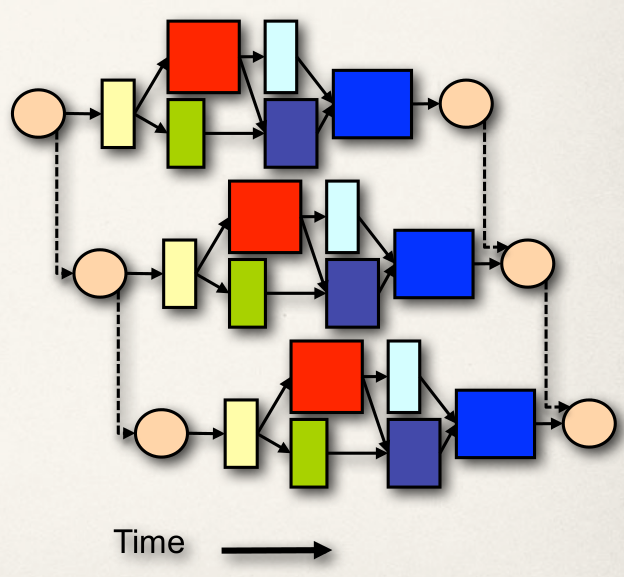
\includegraphics[width=1\textwidth]{figs/gaudi-hive-2.png}
    \end{column}
  \end{columns}

}

\begin{frame}[fragile]
\frametitle{Multithreading in C/C++}


\begin{itemize}
\item parallel programming in \texttt{C++} is \myred{doable}:
\begin{itemize}
\item \verb~C/C++~ \mypurple{\texttt{locks + threads}} (\verb~pthread~,
    \verb~WinThreads~)
\begin{itemize}
\item great performances
\item good generality
\item rather \myred{low productivity}
\end{itemize}
\item multithreaded applications
\begin{itemize}
\item \emph{hard to get right}
\item \emph{hard to \myred{keep} right}
\item \emph{hard to \myred{keep} efficient and optimized across
      releases}
\end{itemize}
\end{itemize}
\end{itemize}

\begin{block}{}

  \begin{center}
 Parallel programming in \texttt{C++} is \alert{doable}, \\
 but \alert{is no \emph{panacea}}
 \end{center}
\end{block}
\end{frame}

\begin{frame}
\frametitle{In a \verb~C++~ world\ldots{}}

\begin{itemize}
\item in \verb~C++03~, we have libraries to help with parallel programming
\begin{itemize}
\item \verb~boost::lambda~
\item \verb~boost::MPL~
\item \verb~boost::thread~
\item Threading Building Blocks (TBB)
\item Concurrent Collections (CnC)
\item \verb~OpenMP~
\item \ldots{}
\end{itemize}
\end{itemize}

\begin{itemize}
\item in \verb~C++11~, we get:
\begin{itemize}
\item $\lambda$ functions (and a new syntax to define them)
\item \verb~std::thread~,
\item \verb~std::future~,
\item \verb~std::promise~
\end{itemize}
\end{itemize}
\end{frame}

\begin{frame}[fragile]
  \frametitle{In a \verb~C++~ world\ldots{}}
  \begin{center}
    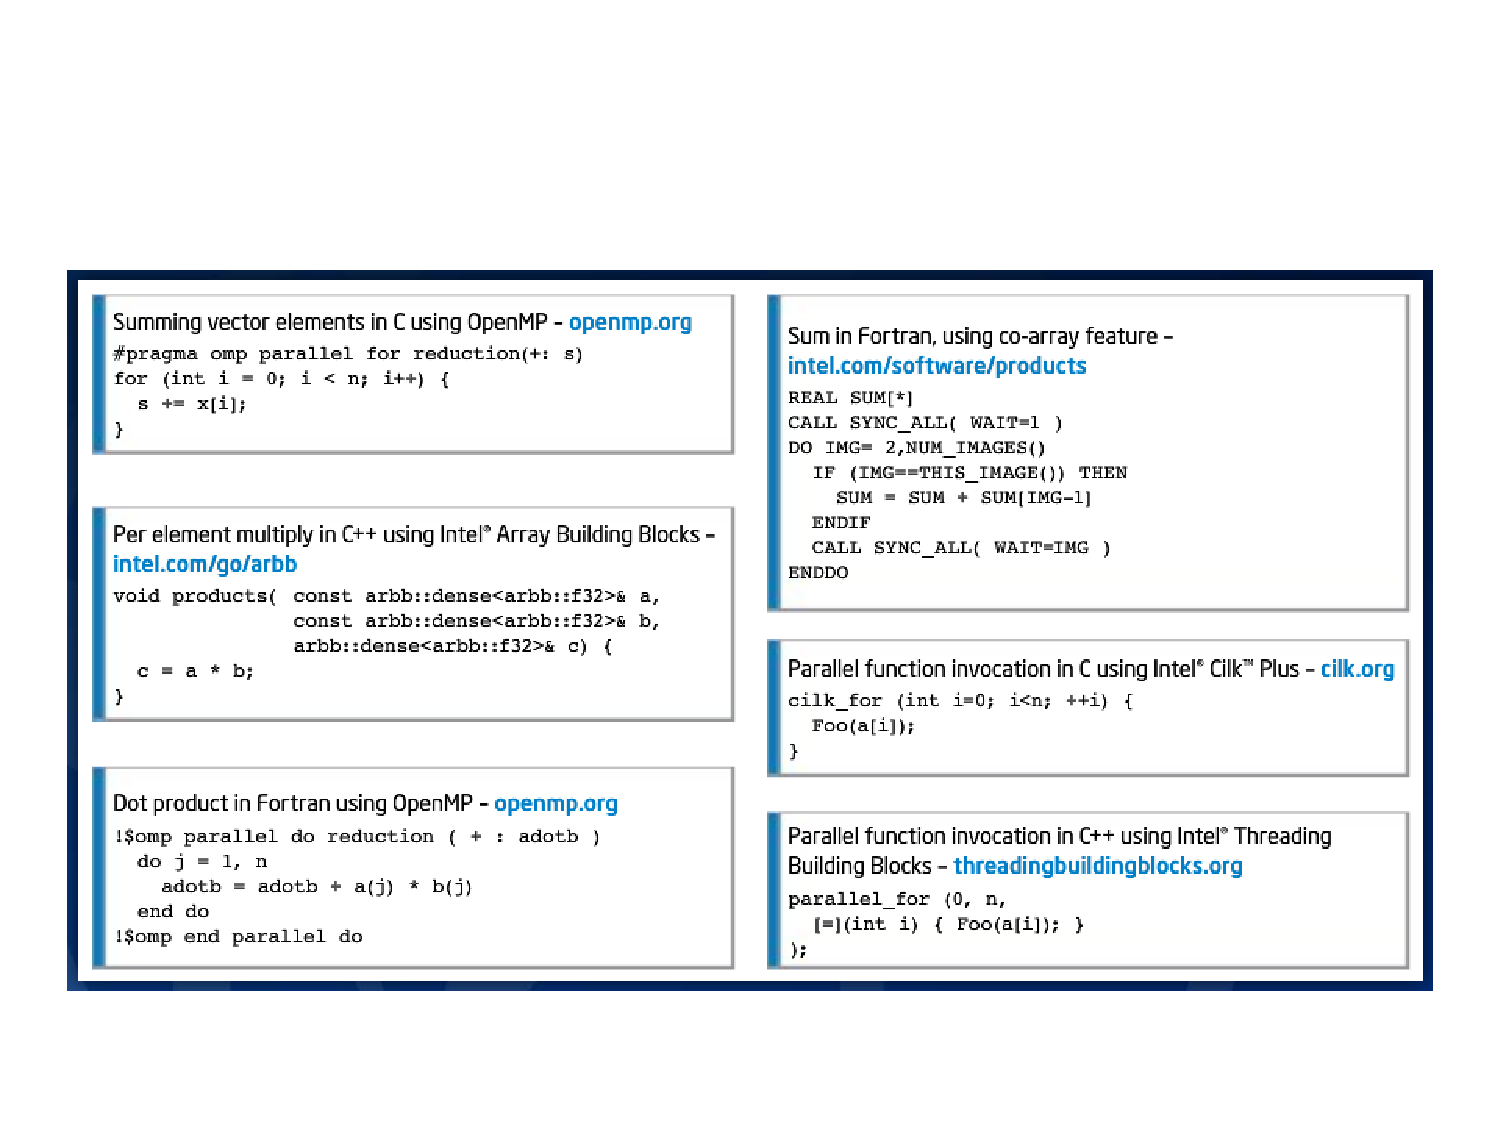
\includegraphics[width=1.\linewidth]{figs/nowak-progs-1.pdf}
  \end{center}
\end{frame}

\begin{frame}[fragile]
  \frametitle{In a \verb~C++~ world\ldots{}}
  \begin{center}
    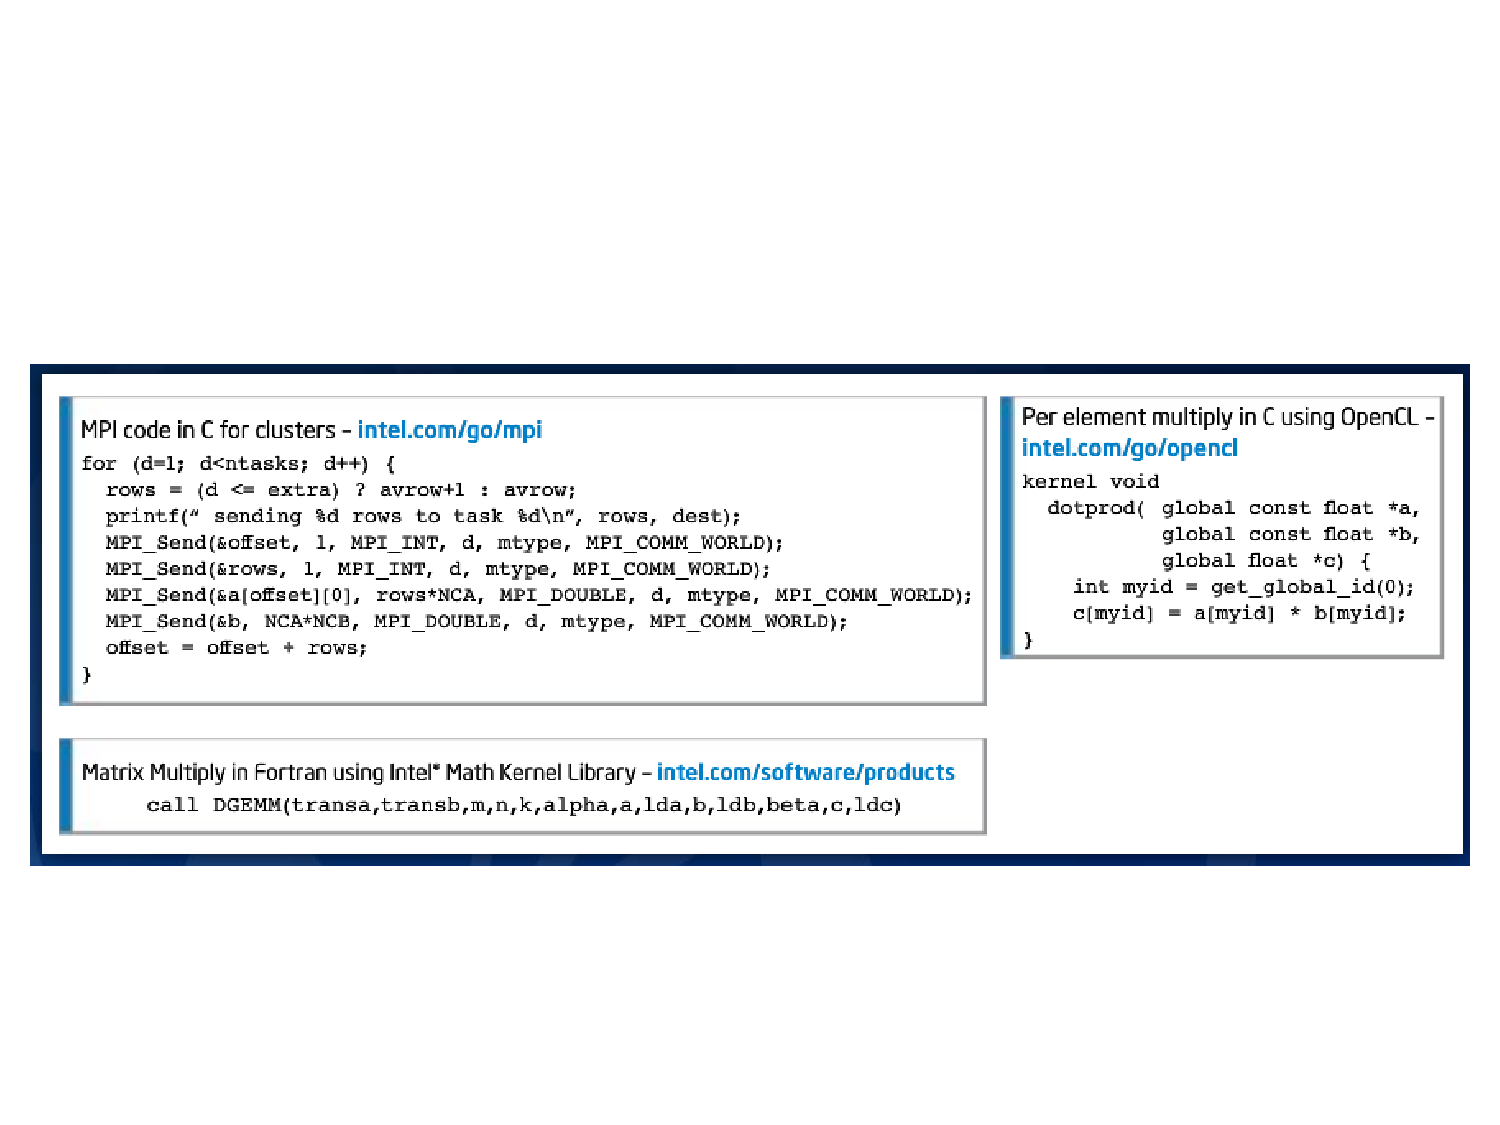
\includegraphics[width=1.\linewidth]{figs/nowak-progs-2.pdf}
  \end{center}

  \begin{block}{}
    \begin{center}
      Jury is still out on which tool is the solution\ldots
    \end{center}
  \end{block}
\end{frame}

\frame{
  \frametitle{Is it (really) tractable ?}

  \begin{center}
    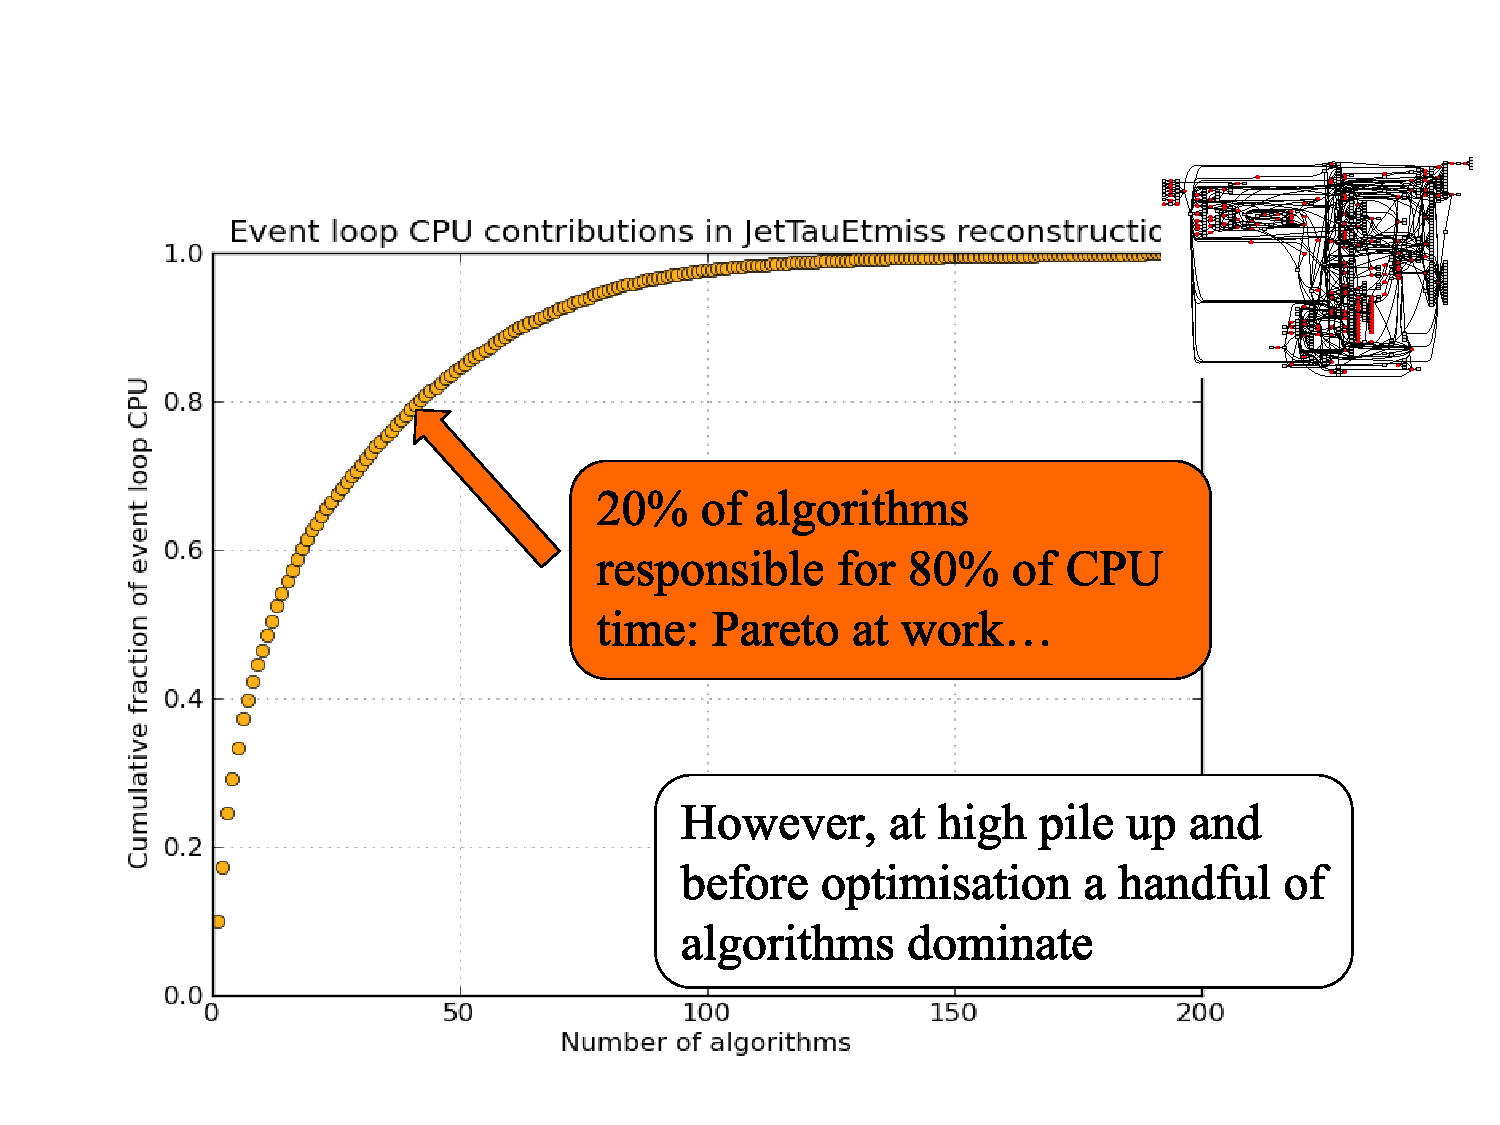
\includegraphics[width=1.\linewidth]{figs/pareto.pdf}
  \end{center}

}

\frame{
  \frametitle{Example: \texttt{LHCb} reconstruction}

  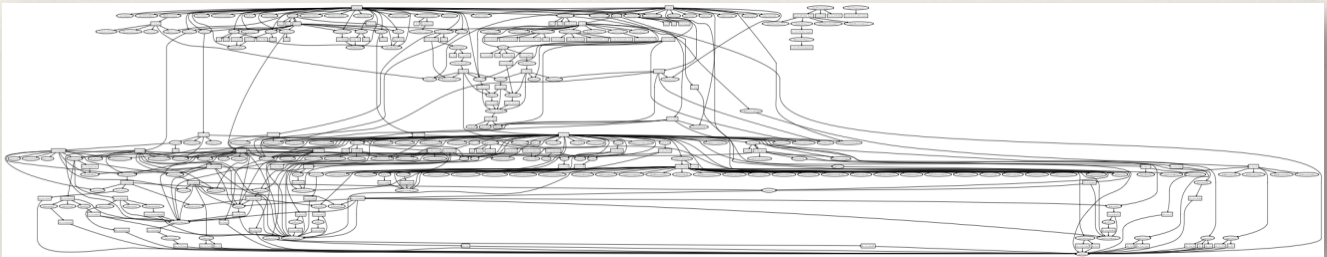
\includegraphics[width=1\textwidth]{figs/dag-brunel.png}

  \begin{columns}
    \begin{column}{0.65\textwidth}
      \begin{block}{}
        \begin{itemize}
          \item DAG of \texttt{Brunel} (214 \texttt{Algorithm}s)
            \begin{itemize}
              \item obtained by instrumenting the existing sequential
                code
              \item probably still missing 'hidden or indirect' dependencies
            \end{itemize}

            \item this can give us an estimate of the potential for
              \emph{concurrency}
              \begin{itemize}
                \item assuming no changes in current reconstruction algorithms
              \end{itemize}
        \end{itemize}
      \end{block}
    \end{column}
    \begin{column}{0.35\textwidth}
      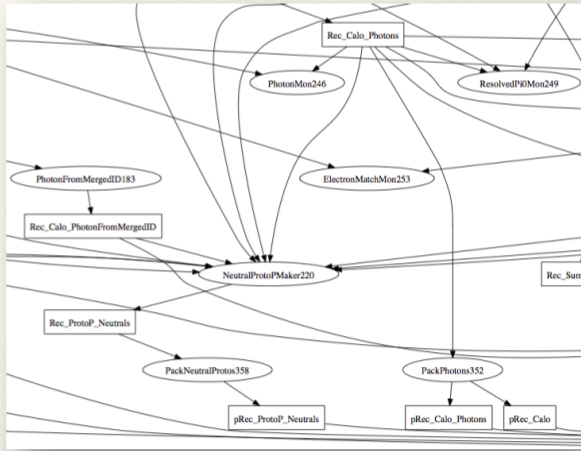
\includegraphics[width=1\textwidth]{figs/dag-brunel-close-up.png}
    \end{column}
  \end{columns}
  
}

\begin{frame}
\frametitle{Implementation and PoC}


Testbed for these developments: \alert{GaudiHive}

  \begin{columns}
    \begin{column}{0.7\textwidth}

      \begin{block}{}
        \begin{itemize}
          \item a LCG/LHCb/ATLAS project
          \item toy framework evolving into a real one
          \begin{itemize}
            \item No real algorithms but CPU crunchers
            \item timing of real workflow reproduced
          \end{itemize}
          \item Schedule algorithm when its inputs are available
        \end{itemize}
      \end{block}

    \end{column}
    \begin{column}{0.35\textwidth}
\begin{figure}
  \begin{center}
    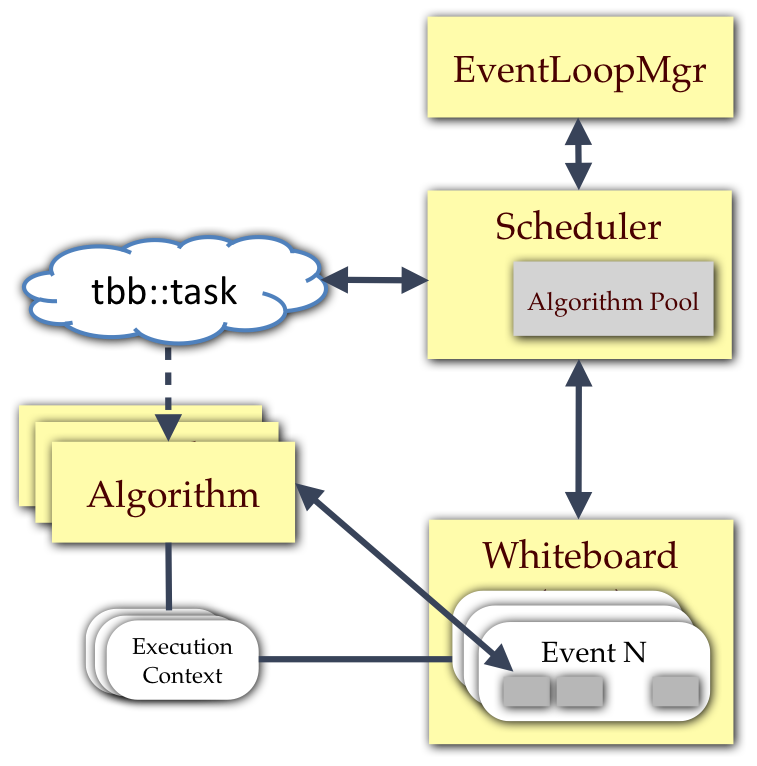
\includegraphics[width=0.95\textwidth]{figs/gaudi-hive.png}
  \end{center}
\end{figure}
    \end{column}
  \end{columns}
\end{frame}

\begin{frame}
\frametitle{Implementation and PoC - II}


  \begin{columns}
    \begin{column}{0.7\textwidth}

      \begin{block}{}
        \begin{itemize}
          \item Multiple events managed simultaneously
          \begin{itemize}
             \item bigger probability to schedule an alg
             \item whiteboard integrated in the \texttt{DataSvc}
             \item \texttt{DataSvc} made thread-safe
          \end{itemize}
          \item Several copies of the same algorithms can coexist
          \begin{itemize}
             \item running on different events
             \item responsibility of \texttt{AlgoPool}
          \end{itemize}
          \item Data specific to execution stored in the \emph{execution context}
        \end{itemize}
      \end{block}

    \end{column}
    \begin{column}{0.35\textwidth}
\begin{figure}
  \begin{center}
    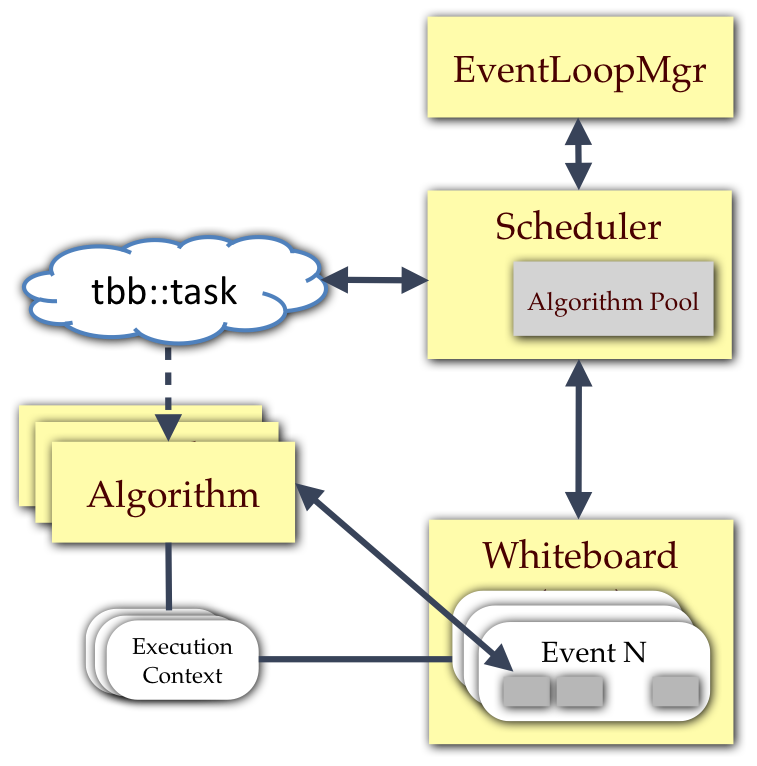
\includegraphics[width=0.95\textwidth]{figs/gaudi-hive.png}
  \end{center}
\end{figure}
    \end{column}
  \end{columns}
\end{frame}

\begin{frame}[fragile]
\frametitle{Implementation notes}


\begin{itemize}
\item task-oriented concurrency handled via \alert{TBB}
\begin{itemize}
\item \textbf{de facto} standard among experiments (\verb~ATLAS~, \verb~CMS~ and \verb~LHCb~)
\item useful concurrent containers and algorithms (\verb~parallel_for~,\ldots{})
\end{itemize}
\item leverage \verb~C++11~ constructs and memory model
\begin{itemize}
\item atomics
\item confortable syntax (range-based \verb~for~ loops, \verb~auto~, \verb~tuples~)
\end{itemize}
\item new algorithm steering to handle dependency graph
\begin{itemize}
\item \alert{opportunity} to streamline/harmonize with \verb~trigger steering~ solution
\end{itemize}
\item thread-safe message service (\verb~TBBMessageService~)
\item work on a thread-safe \verb~ToolSvc~ and \verb~ServiceMgr~
\item auditors ? incidents ?
\end{itemize}
\end{frame}

\frame{
  \frametitle{Test on \texttt{Brunel} workflow}
  \begin{columns}
    \begin{column}{0.5\textwidth}
      \begin{block}{}
        \begin{itemize}
          \item 214 algorithms, real data dependencies, (average) real
            timing
            \begin{itemize}
              \item maximum speedup depends stringly on the workflow chosen
            \end{itemize}
            \item adding more simultaneous events moves the maximum
              concurrency from 3 to 4 with single \texttt{Algorithm}
              instances
            \item increased parallelism when cloning algorithms
              \begin{itemize}
                \item even with a moderate number of events in flight
              \end{itemize}
        \end{itemize}
      \end{block}
    \end{column}
    \begin{column}{0.5\textwidth}
  \begin{center}
    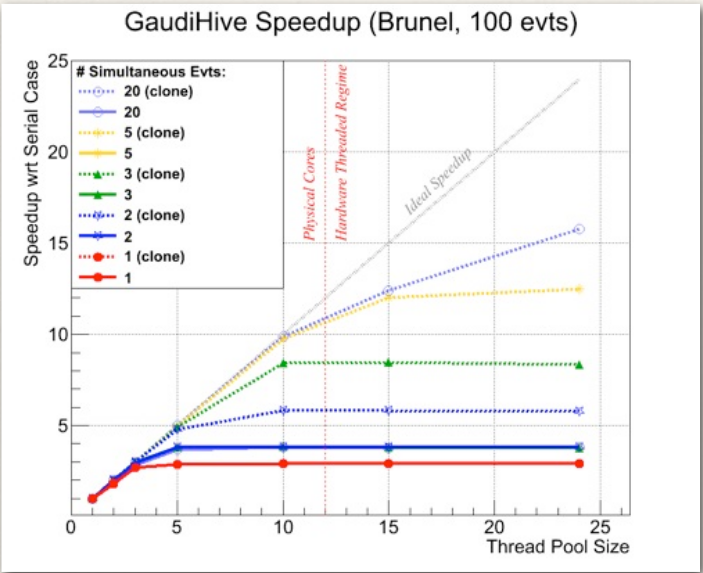
\includegraphics[width=0.95\textwidth]{figs/brunel-perfs.png}
  \end{center}
  \begin{exampleblock}{}
    Test system with 12 physical cores \\ x2 hyperthreads (HT)
    \end{exampleblock}
    \end{column}
  \end{columns}
}

\frame{
  \frametitle{Concurrent \texttt{Gaudi}: status}
  \begin{block}{}
    \begin{itemize}
      \item a prototype of a concurrent \texttt{Gaudi}
        (\texttt{GaudiHive}) has been developed as an evolution (new
        branch in the \texttt{Gaudi} repository)
        \begin{itemize}
          \item able to schedule and run \mypurple{algorithms
            concurrently}
            \item able to run \mypurple{multiple events
              simultaneously}
            \item friendly with \mypurple{sub-event parallelism} if
              using \texttt{TBB}
        \end{itemize}

      \item so far, tested with \texttt{Brunel} reconstruction
        workflow:
        \begin{itemize}
          \item important speedup already been obtained, but no
            \emph{'perfect'} scaling achieved yet
          \item \texttt{Algorithm} cloning increases parallelism,
            keeps \emph{latency} under control
        \end{itemize}

        \item test bench to exercize timings and dependencies for
          other applications:
          \begin{itemize}
            \item \texttt{CMSSW} reconstruction workflow
            \item \texttt{ATLAS} calo-reconstruction
          \end{itemize}
    \end{itemize}
  \end{block}
}

\begin{frame}[fragile]
  \frametitle{In a \verb~C++11~ world\ldots{}}
  \begin{block}{}

    \begin{center}
      \texttt{C++11/C++14} is definitively an improvement, \\
      but the old issues are \myred{still with us\ldots} \\
      (one needs an adequate understanding of the 1300 pages of the \texttt{C++} standard)
    \end{center}
  \end{block}

  \quad

  \begin{itemize}
  \item \alert{build scalability}
    \begin{itemize}
    \item templates
    \item headers
    \item still no modules/packages
      \begin{itemize}
      \item maybe in the next Technical Report ? (2017?)
      \end{itemize}
    \end{itemize}
  \end{itemize}


  \begin{itemize}
  \item \alert{code distribution}
    \begin{itemize}
    \item no \texttt{CPAN}- nor \texttt{PyPI}-like infrastructure (and
      cross-platform) for \texttt{C++}
    \end{itemize}
  \end{itemize}
\end{frame}

\begin{frame}
\frametitle{Time for a new language ?}
\begin{quotation} % \quad

 ``Successful new languages build on existing languages and where possible, support legacy software. C++ grew our of C. java grew out of C++. To the programmer, they are all one continuous family of C languages.''\\
 (T. Mattson)
\end{quotation}
\quad


\begin{itemize}
\item notable exception (which confirms the rule): \alert{python}
\end{itemize}
\begin{alertblock}{\quad}
    Can we have a language:
\begin{itemize}
\item as easy (to learn and use) as \alert{python},
\item as fast (or nearly as fast) as \verb~C/C++/FORTRAN~,
\item with none of the deficiencies of \verb~C++~,
\item and is multicore/manycore friendly ?
\end{itemize}
\end{alertblock}
\end{frame}

\begin{frame}[fragile]
\frametitle{Candidates}
\begin{itemize}
\item \verb~python/pypy~
\item \verb~FORTRAN-2008~
\item \verb~Vala~
\item \verb~Swift~
\item \verb~Rust~
\item \verb~Go~
\item \verb~Chapel~
\item \verb~Scala~
\item \verb~Haskell~
\item \verb~Clojure~
\end{itemize}
\end{frame}

\begin{frame}
\frametitle{\quad}

\begin{center}
  Why not {\texttt Go} ?\\
  \href{http://golang.org}{{\color{blue}golang.org}}
\end{center}
\end{frame}

\begin{frame}[fragile]
\frametitle{Elements of \verb~go~}


\begin{itemize}
\item obligatory \verb~hello world~ example\ldots{}
\end{itemize}

%% FIXME
\begin{block}{}
\begin{center}
  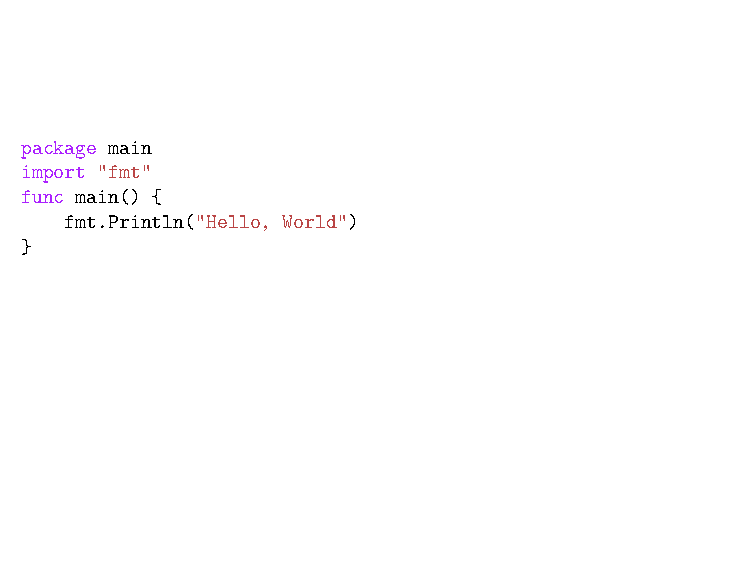
\includegraphics[width=.5\linewidth]{figs/go-hello-world.pdf}
\end{center}
\end{block}
%% \begin{minted}[]{go}
%% package main
%% import "fmt"
%% func main() {
%%     fmt.Println("Hello World")
%% }
%% \end{minted}



\includegraphics[width=.95\linewidth]{figs/golang-logo.png}

\end{frame}

\begin{frame}
\frametitle{Elements of \verb~go~ - II}

\begin{itemize}
  \item founding fathers:
    \begin{itemize}
    \item Russ Cox, Robert Griesemer, Ian Lance Taylor
    \item Rob Pike, Ken Thompson
    \end{itemize}
  \item concurrent, compiled
  \item \alert{garbage collected}
  \item an open-source general programming language
  \item best of both `worlds':
    \begin{itemize}
    \item feel of a \alert{dynamic language}
      \begin{itemize}
      \item limited verbosity thanks to \textbf{type inference system}, map, slices
      \end{itemize}
    \item safety of a \alert{static type system}
    \item compiled down to machine language (so it is fast)
      \begin{itemize}
      \item goal is within 10\% of \alert{C}
      \end{itemize}
    \end{itemize}
  \item \alert{object-oriented} (but w/o classes), \alert{builtin reflection}
  \item first-class functions with \alert{closures}
  \item \myred{duck-typing} \`a la \texttt{python} (but better) thanks to its \myred{interfaces}
\end{itemize}
\end{frame}

\begin{frame}
\frametitle{\verb~Go~ concurrent}
\begin{block}{goroutines}


\begin{itemize}
\item a function executing concurrently as other goroutines \alert{in the same address space}
\item starting a goroutine is done with the \verb~go~ keyword
\begin{itemize}
\item \verb~go myfct(arg1, arg2)~
\end{itemize}
\item growable stack
\begin{itemize}
\item \alert{lightweight threads}
\item starts with a few kB, grows (and shrinks) as needed
\item \mypurple{no stack overflow}
\end{itemize}
\end{itemize}
\end{block}
\end{frame}
\begin{frame}[fragile]
\frametitle{\verb~Go~ concurrent - II}
\begin{block}{channels}


\begin{itemize}
\item provide (type safe) communication and synchronization
\end{itemize}

\begin{center}
  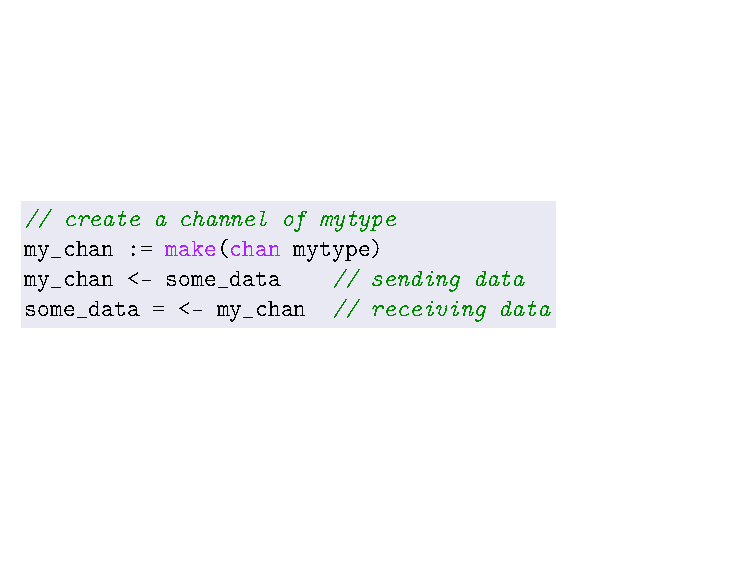
\includegraphics[width=.5\linewidth]{figs/go-chan.pdf}
\end{center}

%% FIXME
%% \begin{minted}[]{go}
%% // create a channel of mytype
%% my_chan := make(chan mytype)
%% my_chan <- some_data    // sending data
%% some_data = <- my_chan  // receiving data
%% \end{minted}




\begin{itemize}
\item \verb~send~ and \verb~receive~ are atomic
\end{itemize}
\end{block}

\begin{alertblock}{\quad}

 \begin{center}
 \emph{
 "Do not communicate by sharing memory; instead, \\
  share memory by communicating"
 }
 \end{center}
\end{alertblock}
\end{frame}

\begin{frame}
\frametitle{Non-elements of \verb~Go~}


\begin{itemize}
\item \alert{no} dynamic libraries (frown upon)
\item \alert{no} dynamic loading (yet)
\begin{itemize}
\item but can either rely on separate processes
\begin{itemize}
\item \verb~IPC~ is made easy \emph{via} the \verb~netchan~ package
\end{itemize}
\item or rebuild executables on the fly
\begin{itemize}
\item \alert{compilation} of \verb~Go~ code is \alert{fast}
\item even faster than \verb~FORTRAN~ and/or \verb~C~
\end{itemize}
\end{itemize}
\item \alert{no} templates/generics
\begin{itemize}
\item still open issue
\item looking for the proper \verb~Go~ -friendly design
\end{itemize}
\item \alert{no} operator overloading
\end{itemize}
\end{frame}

\frame{
  \frametitle{\texttt{go-hep/fads}: real world use case}

  \begin{block}{}
    \begin{itemize}
      \item translated
        \href{https://cp3.irmp.ucl.ac.be/projects/delphes}{{\color{blue}\texttt{C++
              Delphes}}} into \texttt{Go}
        \item \href{https://github.com/go-hep/fads}{{\color{blue}\texttt{go-hep/fads}}}:
          \texttt{Fast Detector Simulation for HEP}
          \item installation:
    \end{itemize}

  \begin{center}
    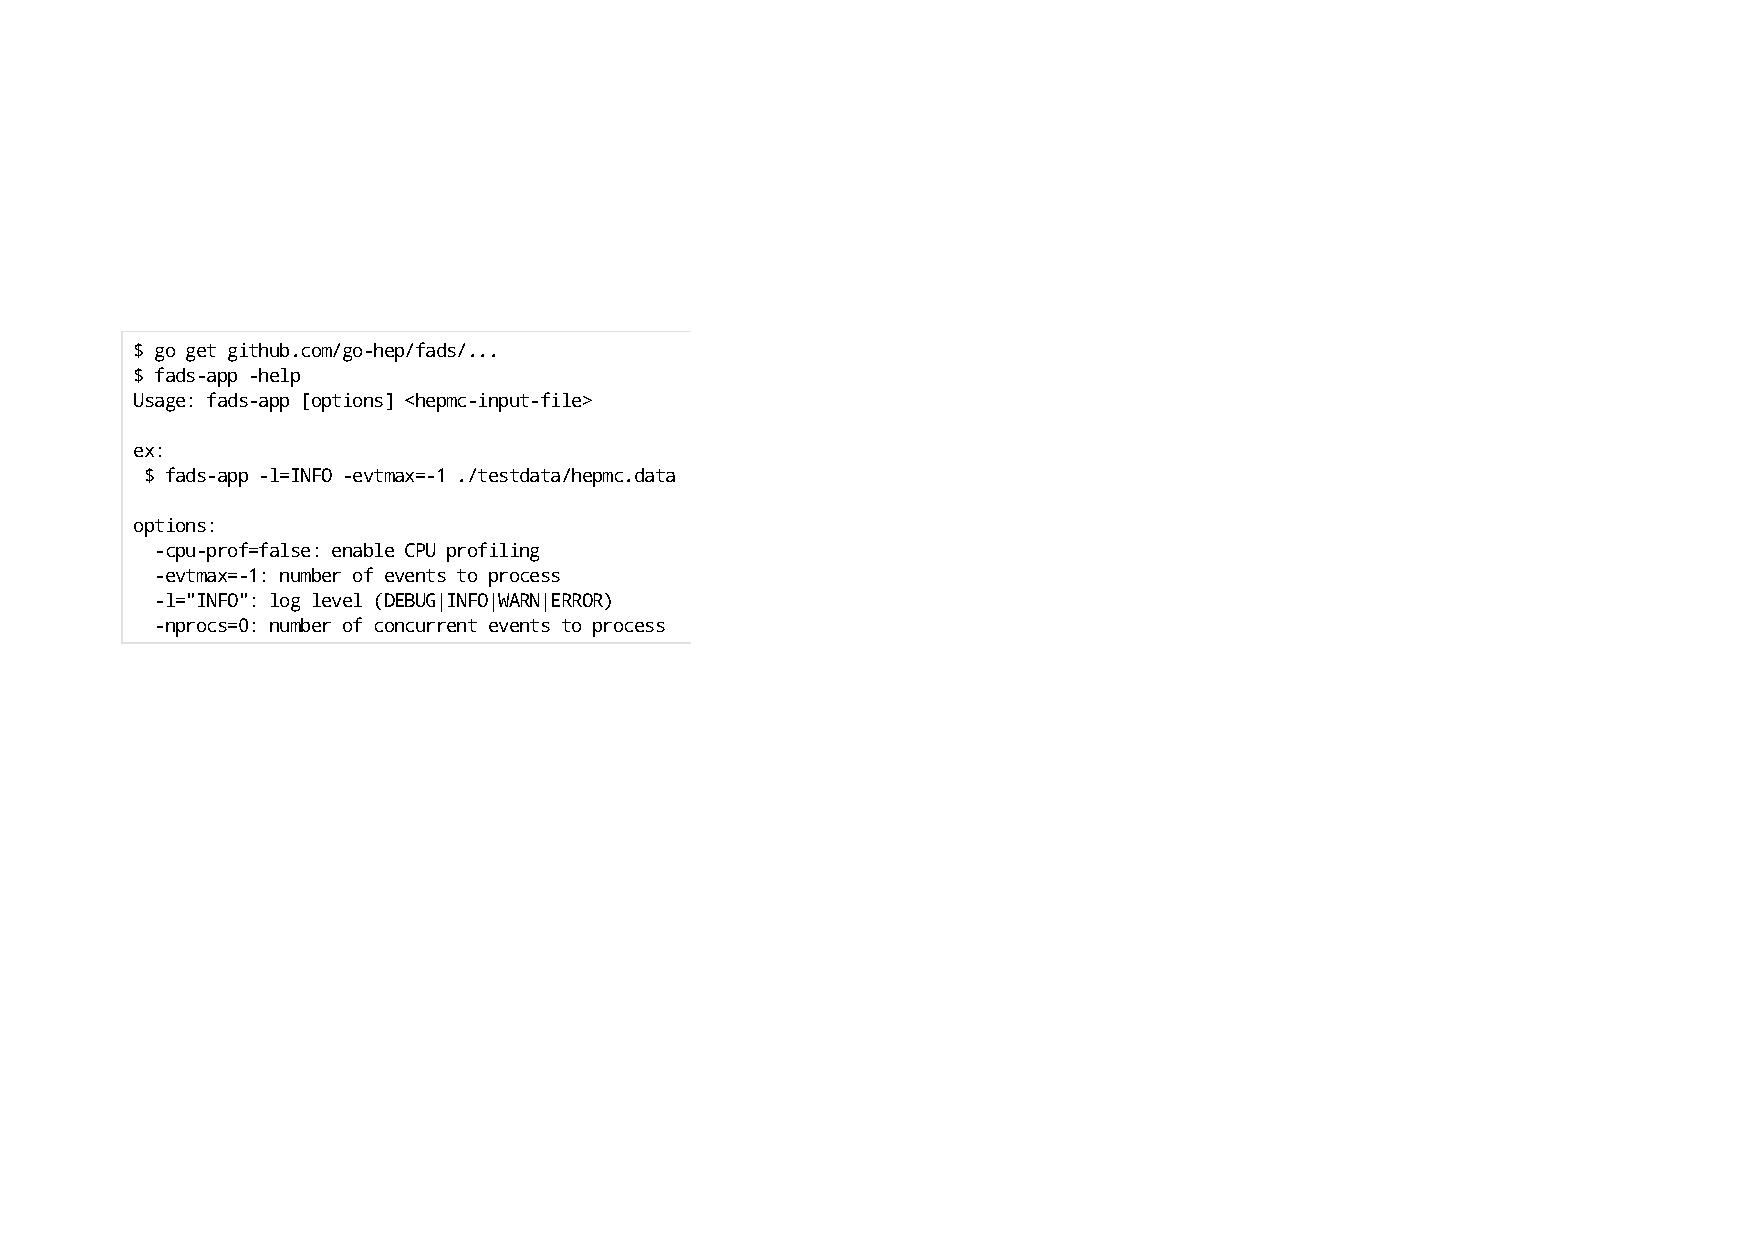
\includegraphics[width=0.65\textwidth]{figs/go-fads-install.pdf}
  \end{center}
  \end{block}
}

\frame{
  \frametitle{\texttt{go-hep/fads} component}

  \begin{block}{}
    \begin{itemize}
    \item a \texttt{HepMC} converter,
    \item particle propagator,
    \item calorimeter simulator,
    \item energy rescaler, momentum smearer,
    \item isolation,
    \item b-tagging, tau-tagging,
    \item jet-finder (reimplementation of \texttt{FastJet} in
      \texttt{Go})
    \item histogram service
    \end{itemize}
  \end{block}

  \begin{exampleblock}{}
    Caveats:
    \begin{itemize}
      \item no real persistency to speak of (\texttt{JSON, ASCII,
        Gob})
      \item jet clustering limited to $N^3$ (slowest and dumbest
        scheme of \texttt{C++-FastJet})
    \end{itemize}
  \end{exampleblock}
}

\frame{
  \frametitle{Performances}
  \begin{block}{}
    \begin{itemize}
      \item good memory footprint scaling (\emph{wrt} \texttt{Delphes}
        and multi-process)
      \item good \texttt{CPU} scaling (\emph{wrt} multi-process)
      \item OK-ish \texttt{CPU} performances \emph{wrt} \texttt{Delphes}
    \end{itemize}
  \end{block}

  \begin{columns}
  \begin{column}{0.5\textwidth}
  \begin{center}
    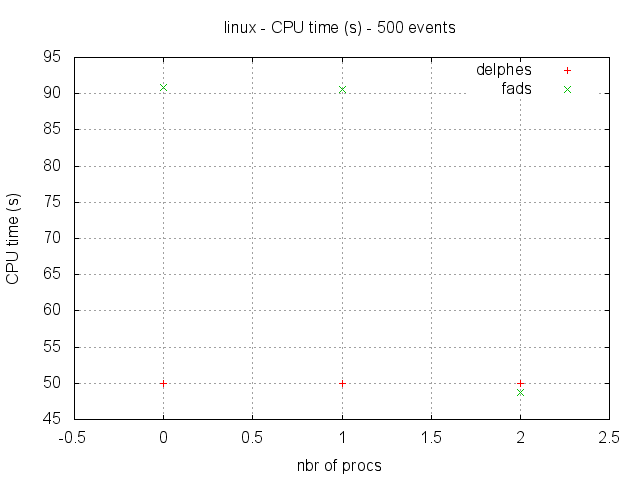
\includegraphics[width=0.65\textwidth]{figs/linux-cpu.png}
  \end{center}
  \begin{center}
    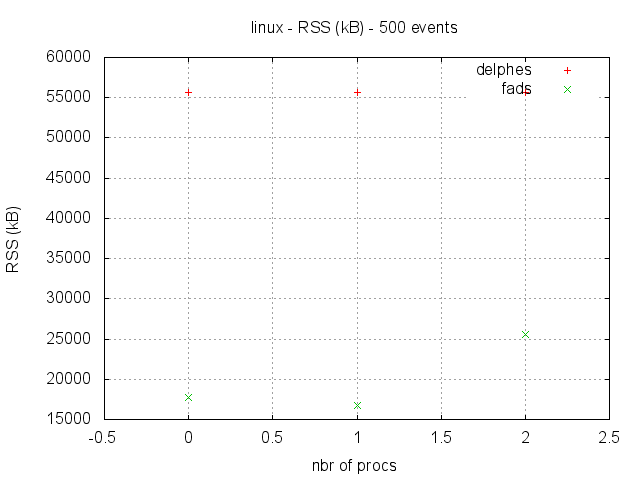
\includegraphics[width=0.65\textwidth]{figs/linux-rss.png}
  \end{center}
  \end{column}
  \begin{column}{0.5\textwidth}
  \begin{center}
    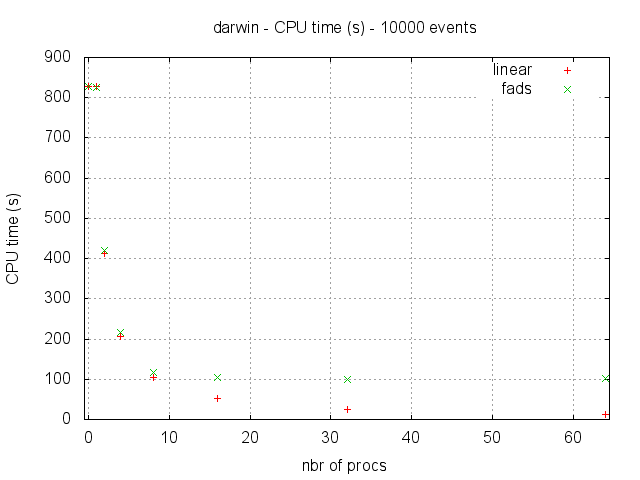
\includegraphics[width=0.65\textwidth]{figs/darwin-cpu.png}
  \end{center}
  \begin{center}
    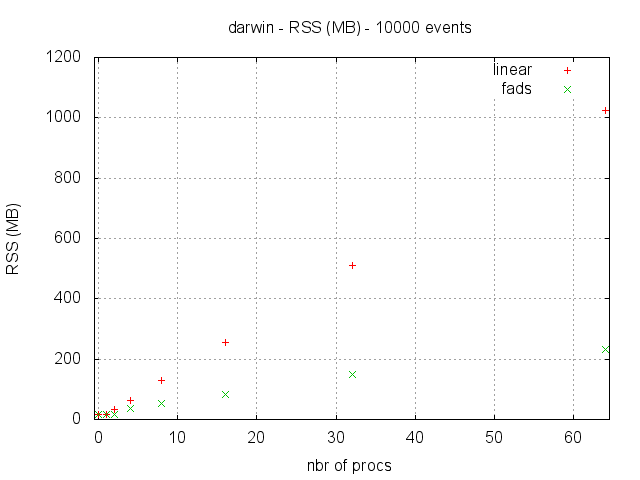
\includegraphics[width=0.65\textwidth]{figs/darwin-rss.png}
  \end{center}
  \end{column}
  \end{columns}
    
}

\begin{frame}
\frametitle{Conclusions}
\begin{center}
\includegraphics[width=0.975\linewidth]{figs/crystal-ball.jpg}
\end{center}
\end{frame}

\begin{frame}[fragile]
\frametitle{Conclusions}


\begin{itemize}
\item Moore's law still observed at the \emph{hardware} level
\begin{itemize}
\item \emph{power wall}
\item \emph{memory wall}
\item \emph{ILP wall}
\end{itemize}
\item \myred{concurrent} and \myred{parallel} programming required to
  efficiently and fully leverage today (and tomorrow)'s \texttt{CPU} architectures
\begin{itemize}
\item \verb~SIMD~ (\verb~SSE~, \verb~AVX~), (auto-)vectorization
\item \emph{data-parallel}
\item \emph{task-parallel}
\item \myred{``think parallel''}
  \item \myred{re-design} code and algorithms in a
    \mypurple{multi-threaded} context
\end{itemize}

\item \verb~ARM~ based servers on the verge of being deployed
\begin{itemize}
\item \verb~AMD~: 2015
\item \verb~Boston Viridis~: \emph{now}
\item better (nimbler) energy consumption (\emph{wrt} traditional \texttt{x86})
\end{itemize}
\item \mypurple{\texttt{Go ?}}
\begin{itemize}
\item \href{http://tour.golang.org}{{\color{blue}tour.golang.org}}
\item tailored for concurrent programming
\item tailored for (easy) \emph{cloud} deployment
\item language and  \emph{runtime} still relatively young but already
  quite robust and performant
\end{itemize}
\end{itemize}
\end{frame}

\frame{
  \begin{center}
    \begin{block}{}
      \begin{center}
        Bonus
      \end{center}
    \end{block}
  \end{center}
}

\frame{
  \begin{center}
    \includegraphics[width=0.99\textwidth]{figs/rousseau-aos-soa.pdf}
  \end{center}
}

\frame{
  \begin{center}
    \includegraphics[width=0.99\textwidth]{figs/rousseau-hsf.pdf}
  \end{center}
}

\frame{
  \begin{center}
    \includegraphics[width=0.99\textwidth]{figs/rousseau-reco-tracks.pdf}
  \end{center}
}

\frame{
  \begin{center}
    \includegraphics[width=0.99\textwidth]{figs/sjarp-mem-cache.pdf}
  \end{center}
}


\end{document}


